\PassOptionsToPackage{unicode=true}{hyperref} % options for packages loaded elsewhere
\PassOptionsToPackage{hyphens}{url}
%
\documentclass[12pt,]{book}
\usepackage{lmodern}
\usepackage{amssymb,amsmath}
\usepackage{ifxetex,ifluatex}
\usepackage{fixltx2e} % provides \textsubscript
\ifnum 0\ifxetex 1\fi\ifluatex 1\fi=0 % if pdftex
  \usepackage[T1]{fontenc}
  \usepackage[utf8]{inputenc}
  \usepackage{textcomp} % provides euro and other symbols
\else % if luatex or xelatex
  \usepackage{unicode-math}
  \defaultfontfeatures{Ligatures=TeX,Scale=MatchLowercase}
\fi
% use upquote if available, for straight quotes in verbatim environments
\IfFileExists{upquote.sty}{\usepackage{upquote}}{}
% use microtype if available
\IfFileExists{microtype.sty}{%
\usepackage[]{microtype}
\UseMicrotypeSet[protrusion]{basicmath} % disable protrusion for tt fonts
}{}
\IfFileExists{parskip.sty}{%
\usepackage{parskip}
}{% else
\setlength{\parindent}{0pt}
\setlength{\parskip}{6pt plus 2pt minus 1pt}
}
\usepackage{hyperref}
\hypersetup{
            pdftitle={How to fit an animal model},
            pdfauthor={Julien Martin},
            pdfborder={0 0 0},
            breaklinks=true}
\urlstyle{same}  % don't use monospace font for urls
\usepackage{color}
\usepackage{fancyvrb}
\newcommand{\VerbBar}{|}
\newcommand{\VERB}{\Verb[commandchars=\\\{\}]}
\DefineVerbatimEnvironment{Highlighting}{Verbatim}{commandchars=\\\{\}}
% Add ',fontsize=\small' for more characters per line
\usepackage{framed}
\definecolor{shadecolor}{RGB}{248,248,248}
\newenvironment{Shaded}{\begin{snugshade}}{\end{snugshade}}
\newcommand{\AlertTok}[1]{\textcolor[rgb]{0.94,0.16,0.16}{#1}}
\newcommand{\AnnotationTok}[1]{\textcolor[rgb]{0.56,0.35,0.01}{\textbf{\textit{#1}}}}
\newcommand{\AttributeTok}[1]{\textcolor[rgb]{0.77,0.63,0.00}{#1}}
\newcommand{\BaseNTok}[1]{\textcolor[rgb]{0.00,0.00,0.81}{#1}}
\newcommand{\BuiltInTok}[1]{#1}
\newcommand{\CharTok}[1]{\textcolor[rgb]{0.31,0.60,0.02}{#1}}
\newcommand{\CommentTok}[1]{\textcolor[rgb]{0.56,0.35,0.01}{\textit{#1}}}
\newcommand{\CommentVarTok}[1]{\textcolor[rgb]{0.56,0.35,0.01}{\textbf{\textit{#1}}}}
\newcommand{\ConstantTok}[1]{\textcolor[rgb]{0.00,0.00,0.00}{#1}}
\newcommand{\ControlFlowTok}[1]{\textcolor[rgb]{0.13,0.29,0.53}{\textbf{#1}}}
\newcommand{\DataTypeTok}[1]{\textcolor[rgb]{0.13,0.29,0.53}{#1}}
\newcommand{\DecValTok}[1]{\textcolor[rgb]{0.00,0.00,0.81}{#1}}
\newcommand{\DocumentationTok}[1]{\textcolor[rgb]{0.56,0.35,0.01}{\textbf{\textit{#1}}}}
\newcommand{\ErrorTok}[1]{\textcolor[rgb]{0.64,0.00,0.00}{\textbf{#1}}}
\newcommand{\ExtensionTok}[1]{#1}
\newcommand{\FloatTok}[1]{\textcolor[rgb]{0.00,0.00,0.81}{#1}}
\newcommand{\FunctionTok}[1]{\textcolor[rgb]{0.00,0.00,0.00}{#1}}
\newcommand{\ImportTok}[1]{#1}
\newcommand{\InformationTok}[1]{\textcolor[rgb]{0.56,0.35,0.01}{\textbf{\textit{#1}}}}
\newcommand{\KeywordTok}[1]{\textcolor[rgb]{0.13,0.29,0.53}{\textbf{#1}}}
\newcommand{\NormalTok}[1]{#1}
\newcommand{\OperatorTok}[1]{\textcolor[rgb]{0.81,0.36,0.00}{\textbf{#1}}}
\newcommand{\OtherTok}[1]{\textcolor[rgb]{0.56,0.35,0.01}{#1}}
\newcommand{\PreprocessorTok}[1]{\textcolor[rgb]{0.56,0.35,0.01}{\textit{#1}}}
\newcommand{\RegionMarkerTok}[1]{#1}
\newcommand{\SpecialCharTok}[1]{\textcolor[rgb]{0.00,0.00,0.00}{#1}}
\newcommand{\SpecialStringTok}[1]{\textcolor[rgb]{0.31,0.60,0.02}{#1}}
\newcommand{\StringTok}[1]{\textcolor[rgb]{0.31,0.60,0.02}{#1}}
\newcommand{\VariableTok}[1]{\textcolor[rgb]{0.00,0.00,0.00}{#1}}
\newcommand{\VerbatimStringTok}[1]{\textcolor[rgb]{0.31,0.60,0.02}{#1}}
\newcommand{\WarningTok}[1]{\textcolor[rgb]{0.56,0.35,0.01}{\textbf{\textit{#1}}}}
\usepackage{longtable,booktabs}
% Fix footnotes in tables (requires footnote package)
\IfFileExists{footnote.sty}{\usepackage{footnote}\makesavenoteenv{longtable}}{}
\usepackage{graphicx,grffile}
\makeatletter
\def\maxwidth{\ifdim\Gin@nat@width>\linewidth\linewidth\else\Gin@nat@width\fi}
\def\maxheight{\ifdim\Gin@nat@height>\textheight\textheight\else\Gin@nat@height\fi}
\makeatother
% Scale images if necessary, so that they will not overflow the page
% margins by default, and it is still possible to overwrite the defaults
% using explicit options in \includegraphics[width, height, ...]{}
\setkeys{Gin}{width=\maxwidth,height=\maxheight,keepaspectratio}
\setlength{\emergencystretch}{3em}  % prevent overfull lines
\providecommand{\tightlist}{%
  \setlength{\itemsep}{0pt}\setlength{\parskip}{0pt}}
\setcounter{secnumdepth}{5}
% Redefines (sub)paragraphs to behave more like sections
\ifx\paragraph\undefined\else
\let\oldparagraph\paragraph
\renewcommand{\paragraph}[1]{\oldparagraph{#1}\mbox{}}
\fi
\ifx\subparagraph\undefined\else
\let\oldsubparagraph\subparagraph
\renewcommand{\subparagraph}[1]{\oldsubparagraph{#1}\mbox{}}
\fi

% set default figure placement to htbp
\makeatletter
\def\fps@figure{htbp}
\makeatother

%\usepackage{booktabs}
\usepackage{ctable}
\usepackage{fancyhdr}
\usepackage{float}
\usepackage[margin=2cm]{geometry}

\floatplacement{figure}{H}

%\usepackage[sf,bf]{titlesec}

\hypersetup{colorlinks=true, urlcolor=blue}

\renewcommand{\chaptername}{Chapitre}
\renewcommand{\contentsname}{Table des Matières}
\renewcommand{\partname}{Partie}

\usepackage{framed,color}
\definecolor{incolor}{RGB}{240,240,240}
\definecolor{outcolor}{RGB}{248,248,248}

\renewcommand{\textfraction}{0.05}
\renewcommand{\topfraction}{0.8}
\renewcommand{\bottomfraction}{0.8}
\renewcommand{\floatpagefraction}{0.75}

%\renewenvironment{quote}{\begin{VF}}{\end{VF}}

\ifxetex
 \usepackage{letltxmacro}
 \setlength{\XeTeXLinkMargin}{1pt}
 \LetLtxMacro\SavedIncludeGraphics\includegraphics
 \def\includegraphics#1#{% #1 catches optional stuff (star/opt. arg.)
   \IncludeGraphicsAux{#1}%
 }%
 \newcommand*{\IncludeGraphicsAux}[2]{%
   \XeTeXLinkBox{%
     \SavedIncludeGraphics#1{#2}%
   }%
 }%
\fi

\makeatletter
\newenvironment{kframe}{%
\medskip{}
\setlength{\fboxsep}{.8em}
\def\at@end@of@kframe{}%
\ifinner\ifhmode%
 \def\at@end@of@kframe{\end{minipage}}%
 \begin{minipage}{\columnwidth}%
\fi\fi%
\def\FrameCommand##1{\hskip\@totalleftmargin \hskip-\fboxsep
\colorbox{incolor}{##1}\hskip-\fboxsep
    % There is no \\@totalrightmargin, so:
    \hskip-\linewidth \hskip-\@totalleftmargin \hskip\columnwidth}%
\MakeFramed {\advance\hsize-\width
  \@totalleftmargin\z@ \linewidth\hsize
  \@setminipage}}%
{\par\unskip\endMakeFramed%
\at@end@of@kframe}
\makeatother

\makeatletter
\@ifundefined{Shaded}{
}{\renewenvironment{Shaded}{\begin{kframe}}{\end{kframe}}}
\makeatother

% \let\oldverbatim\verbatim
% \renewenvironment{Shaded}{\vspace{0.2cm}\begin{kframe}}{\end{kframe}}
% \renewenvironment{verbatim}{\begin{shaded}\begin{oldverbatim}}{\end{oldverbatim}\end{shaded}}

\newenvironment{rmdblock}[1]
 {
 \begin{itemize}
 \renewcommand{\labelitemi}{
   \raisebox{-.7\height}[0pt][0pt]{
     {\setkeys{Gin}{width=3em,keepaspectratio}\includegraphics{images/#1}}
   }
 }
 \begin{kframe}
 \setlength{\fboxsep}{1em}
 \item
 }
 {
 \end{kframe}
 \end{itemize}
 }
\newenvironment{rmdnote}
  {\begin{rmdblock}{note}}
  {\end{rmdblock}}
\newenvironment{rmdcaution}
  {\begin{rmdblock}{caution}}
  {\end{rmdblock}}
\newenvironment{rmdimportant}
  {\begin{rmdblock}{important}}
  {\end{rmdblock}}
\newenvironment{rmdtip}
  {\begin{rmdblock}{tip}}
  {\end{rmdblock}}
\newenvironment{rmdwarning}
  {\begin{rmdblock}{warning}}
  {\end{rmdblock}}
\newenvironment{rmdcode}
  {\begin{rmdblock}{screen}}
  {\end{rmdblock}}

\usepackage{makeidx}
\makeindex

\urlstyle{tt}

\usepackage{amsthm}
\makeatletter
\def\thm@space@setup{%
  \thm@preskip=8pt plus 2pt minus 4pt
  \thm@postskip=\thm@preskip
}
\makeatother

% \frontmatter
\usepackage[]{natbib}
\bibliographystyle{apalike}

\title{How to fit an animal model}
\providecommand{\subtitle}[1]{}
\subtitle{An ecologist guide}
\author{Julien Martin}
\date{12-02-2021}

\begin{document}
\maketitle

%\cleardoublepage\newpage\thispagestyle{empty}\null
%\cleardoublepage\newpage\thispagestyle{empty}\null
%\cleardoublepage\newpage
%\thispagestyle{empty}
%\begin{center}
%
\includegraphics{images/missing.png}
%\end{center}

%\setlength{\abovedisplayskip}{-5pt}
%\setlength{\abovedisplayshortskip}{-5pt}

{
\setcounter{tocdepth}{1}
\tableofcontents
}
\hypertarget{preface}{%
\chapter*{Preface}\label{preface}}
\addcontentsline{toc}{chapter}{Preface}

This book is a collection of tutorial from the excellent paper by \citep{wilson2010}.
Instead of just copy pasting the tutorial in a bookdown format, the tutorials have been updated to work with the newest version of the softwares and extended to present other softwares.
\textbf{However, this is still a work in progress.}

\hypertarget{contributors}{%
\subsection*{Contributors}\label{contributors}}
\addcontentsline{toc}{subsection}{Contributors}

List of people who contributed to update and extend tutorials:

\begin{itemize}
\tightlist
\item
  Eric Postma
\item
  Julien Martin
\end{itemize}

\hypertarget{intro}{%
\chapter{Introduction}\label{intro}}

The book is provides a series of tutorials (and accompanying data files) to fit animal model in \texttt{R} using different packages (\texttt{ASReml-R}, \texttt{gremlin}, \texttt{MCMCglmm} and \texttt{brms}) .
You will need to carefully follow the instructions below to download the data files and install the R packages.
Before beginning the tutorial, we assume the reader has successfully installed the chosen R package on their computer and has saved the required data files to an appropriate directory from which they will be read.
Full instructions for how to do this are provided with software distributions.

To work though the different tutorial I would recommend to create a folder where you will save your different \texttt{R} scripts for the tutorials. In addition, I recommand to create a subfolder \texttt{data} to save the files needed.

\hypertarget{data}{%
\section{Data}\label{data}}

\hypertarget{data-files}{%
\subsection{Data files}\label{data-files}}

You will need to download 3 data files for the tutorial in \texttt{R}:

\begin{itemize}
\tightlist
\item
  gryphon.csv: data on gryphon birth weight
\item
  gryphonRM.csv: data
\item
  gryphonped.csv
\end{itemize}

In addition, some models presented in the tutorials can take a while to run (sometimes \textgreater{} 1 hour), thus we are also providing model the model outputs to allow you continue the tutorial without waiting for the model to run.

The files are available \href{https://github.com/JulienGAMartin/wam_tuto/tree/master/data}{here}

I recommend to save the data and Rdata files in a subfolder \texttt{data} in the folder you will use as your working directory for R and where you will save your R scripts. It should be noted that the tutorial are using this structure to read or save data.

\hypertarget{notes-on-data-and-pedigree}{%
\subsection{Notes on data and pedigree}\label{notes-on-data-and-pedigree}}

It is always important to take time to think carefully about the strengths and potential limitations of your pedigree information before embarking on quantitative genetic analyses. Pedigree Viewer, written by Brian Kinghorn, is an extremely useful application for visualising pedigrees, and can be downloaded from: \url{http://www-personal.une.edu.au/~bkinghor/pedigree.htm}. \texttt{Pedantics} an R package written by Michael Morrissey and distributed through CRAN (\url{http://cran.r-project.org/}) can also be used for this and offers some nice additional features for visualising pedigree structures and generating associated statistics. Before you begin running through the tutorials, we advise taking a moment to look at the pedigree files provided with them using Pedigree Viewer or Pedantics.

\hypertarget{r}{%
\section{R}\label{r}}

describe R Briefly
You should check that you have the most current version of R and R packages. You can check the number of the current version on CRAN. If you need to update (or install) R packages, use \texttt{install.packages()} and follow the prompted instructions.

\hypertarget{r-packages}{%
\subsection{R packages}\label{r-packages}}

describe briefly the differnet r packages indicate how to load and install provide warning on cost and complexity indicating that we are just touching the surface of what they can do

\hypertarget{asreml-r}{%
\subsubsection{asreml-r}\label{asreml-r}}

ASReml-R is commercial software published by VSN international (\url{http://www.vsni.co.uk/software/asreml/}).

\hypertarget{gremlin}{%
\subsubsection{gremlin}\label{gremlin}}

\texttt{gremlin} is a little monster appearing if you wet a mugwai and feed it after midnight. It is also a great and promising software to fit mixed models using a freuqentist approach.

\hypertarget{mcmcglmm}{%
\subsubsection{MCMCglmm}\label{mcmcglmm}}

\texttt{MCMCglmm} is an R package for Bayesian mixed model analysis written by Jarrod Hadfield. It is
freeware distributed through CRAN (\url{http://cran.r-project.org/}). Information about the package, together
with a user manual and vignettes are available at \url{http://cran.r-project.org/web/packages/MCMCglmm/index.html} .
Reference: \citep[\citet{R-MCMCglmm}]{MCMCglmm2010}.

This module provides some information that applies to MCMCglmm-based analyses in general, but that will not be included in other tutorials.
Most importantly, this applies to some of the simplest waysof determining the performance of a run using MCMCglmm, i.e., verification of the validity of of the posterior distribution.
This tutorial is not a substitute for working through the MCMCglmm course notes, which is available from CRAN (the Comprehensive R ArchiveNetwork, \url{http://cran.r-project.org/}, or can be accessed in R using the command vignette(``CourseNotes'',``MCMCglmm'')).
These tutorials do not introduce one of the main advantages of using MCMCglmm for analyses of data from natural populations -the ability to properly model non-normal responses.
These capabilities are introduced inthe documentation that is distributed with MCMCglmm, and available from CRAN.

\hypertarget{brms}{%
\subsubsection{brms}\label{brms}}

\texttt{brms} provides an interface to fit Bayesian generalized multivariate (non-)linear multilevel models using \texttt{Stan}, which is a C++ package for obtaining full Bayesian inference (see \url{https://mc-stan.org/}).
The formula syntax is an extended version of the syntax applied in the `lme4' package to provide a familiar and simple interface for performing regression analyses.

It should be noted that if \texttt{brms} is able to fit animal model the parametrization used based on Kroeneker products is not the most efficient and can take quite longer than using a DAG parametrisation directly in \texttt{stan}.

\hypertarget{univariate-animal-model}{%
\chapter{Univariate animal model}\label{univariate-animal-model}}

This tutorial will demonstrate how to run a univariate animal model to estimate genetic variance in birth weight in the mighty gryphons.

\hypertarget{scenario-and-data}{%
\section{Scenario and data}\label{scenario-and-data}}

\hypertarget{scenario}{%
\subsection{Scenario}\label{scenario}}

In a population of gryphons there is strong positive selection on birth weight with heavier born individuals having, on average higher fitness. To find out whether increased birth weight will evolve in response to the selection, and if so how quickly, we want to estimate the heritability of birth weight.

\hypertarget{data-files-1}{%
\subsection{Data files}\label{data-files-1}}

Open \texttt{gryphonped.csv} and \texttt{gryphon.csv} in your text editor. The structure and contents of these files is fairly self-explanatory. The pedigree file \texttt{gryphonped.csv} contains three columns containing unique IDs that correspond to each animal, its father, and its mother. Note that this is a multigenerational pedigree, with the earliest generation (for which parentage information is necessarily missing) at the beginning of the file. For later-born individuals maternal identities are all known but paternity information is incomplete (a common situation in real world applications).
The phenotype data, as well as additional factors and covariates that we may wish to include in our model are contained in \texttt{gryphon.csv}. Columns correspond to individual identity (\texttt{animal}), maternal identity (\texttt{mother}), year of birth (\texttt{byear}), sex (\texttt{sex}, where \texttt{1} is female and \texttt{2} is male), birth weight (\texttt{bwt}), and tarsus length (\texttt{tarsus}). Each row of the data file contains a record for a different offspring individual. Note that all individuals included in the data file must be included as offspring in the pedigree file.

We can read teh data file, using \texttt{read.csv()} which consider by default that \texttt{NA} is the symbol for missing values and that the first line of the file contains the column headers.

It is a good idea to make sure that all variables are correctly assigned as numeric or factors:

\begin{Shaded}
\begin{Highlighting}[]
\NormalTok{gryphon}\OperatorTok{$}\NormalTok{animal <-}\StringTok{ }\KeywordTok{as.factor}\NormalTok{(gryphon}\OperatorTok{$}\NormalTok{animal)}
\NormalTok{gryphon}\OperatorTok{$}\NormalTok{mother <-}\StringTok{ }\KeywordTok{as.factor}\NormalTok{(gryphon}\OperatorTok{$}\NormalTok{mother)}
\NormalTok{gryphon}\OperatorTok{$}\NormalTok{byear <-}\StringTok{ }\KeywordTok{as.factor}\NormalTok{(gryphon}\OperatorTok{$}\NormalTok{byear)}
\NormalTok{gryphon}\OperatorTok{$}\NormalTok{sex <-}\StringTok{ }\KeywordTok{as.factor}\NormalTok{(gryphon}\OperatorTok{$}\NormalTok{sex)}
\NormalTok{gryphon}\OperatorTok{$}\NormalTok{bwt <-}\StringTok{ }\KeywordTok{as.numeric}\NormalTok{(gryphon}\OperatorTok{$}\NormalTok{bwt)}
\NormalTok{gryphon}\OperatorTok{$}\NormalTok{tarsus <-}\StringTok{ }\KeywordTok{as.numeric}\NormalTok{(gryphon}\OperatorTok{$}\NormalTok{tarsus)}
\end{Highlighting}
\end{Shaded}

Similarly we can read in the pedigree file, using \texttt{read.csv()} which consider by default that \texttt{NA} is the symbol for missing values and that the first line of the file contains the column headers.

\begin{verbatim}
## 'data.frame':    1309 obs. of  3 variables:
##  $ id    : int  1306 1304 1298 1293 1290 1288 1284 1283 1282 1278 ...
##  $ father: int  NA NA NA NA NA NA NA NA NA NA ...
##  $ mother: int  NA NA NA NA NA NA NA NA NA NA ...
\end{verbatim}

\begin{Shaded}
\begin{Highlighting}[]
\NormalTok{gryphonped}\OperatorTok{$}\NormalTok{id <-}\StringTok{ }\KeywordTok{as.factor}\NormalTok{(gryphonped}\OperatorTok{$}\NormalTok{id)}
\NormalTok{gryphonped}\OperatorTok{$}\NormalTok{father <-}\StringTok{ }\KeywordTok{as.factor}\NormalTok{(gryphonped}\OperatorTok{$}\NormalTok{father)}
\NormalTok{gryphonped}\OperatorTok{$}\NormalTok{mother <-}\StringTok{ }\KeywordTok{as.factor}\NormalTok{(gryphonped}\OperatorTok{$}\NormalTok{mother)}
\end{Highlighting}
\end{Shaded}

Now that we have imported the data and the pedigree file, we are ready to fit an animal model.

\hypertarget{asreml-r-1}{%
\section{Asreml-R}\label{asreml-r-1}}

\hypertarget{running-the-model}{%
\subsection{Running the model}\label{running-the-model}}

First we need to load the \texttt{asreml} library:

\begin{Shaded}
\begin{Highlighting}[]
\KeywordTok{library}\NormalTok{(asreml)}
\end{Highlighting}
\end{Shaded}

To be able to fit an animal model Asreml-r needs (the inverse of) the relationship matrix:

\begin{Shaded}
\begin{Highlighting}[]
\NormalTok{ainv <-}\StringTok{ }\KeywordTok{ainverse}\NormalTok{(gryphonped)}
\end{Highlighting}
\end{Shaded}

We are now ready to specify our first model:

\begin{Shaded}
\begin{Highlighting}[]
\NormalTok{model1 <-}\StringTok{ }\KeywordTok{asreml}\NormalTok{(}
  \DataTypeTok{fixed =}\NormalTok{ bwt }\OperatorTok{~}\StringTok{ }\DecValTok{1}\NormalTok{, }\DataTypeTok{random =} \OperatorTok{~}\StringTok{ }\KeywordTok{vm}\NormalTok{(animal, ainv),}
  \DataTypeTok{residual =} \OperatorTok{~}\StringTok{ }\KeywordTok{idv}\NormalTok{(units),}
  \DataTypeTok{data =}\NormalTok{ gryphon,}
  \DataTypeTok{na.action =} \KeywordTok{na.method}\NormalTok{(}\DataTypeTok{x =} \StringTok{"omit"}\NormalTok{, }\DataTypeTok{y =} \StringTok{"omit"}\NormalTok{)}
\NormalTok{)}
\end{Highlighting}
\end{Shaded}

\begin{verbatim}
## Model fitted using the sigma parameterization.
## ASReml 4.1.0 Fri Feb 12 17:19:29 2021
##           LogLik        Sigma2     DF     wall    cpu
##  1     -4128.454           1.0    853 17:19:29    0.0
##  2     -3284.272           1.0    853 17:19:29    0.0
##  3     -2354.992           1.0    853 17:19:29    0.0
##  4     -1710.357           1.0    853 17:19:29    0.0
##  5     -1363.555           1.0    853 17:19:29    0.0
##  6     -1263.516           1.0    853 17:19:29    0.0
##  7     -1247.854           1.0    853 17:19:29    0.0
##  8     -1247.185           1.0    853 17:19:29    0.0
##  9     -1247.183           1.0    853 17:19:29    0.0
\end{verbatim}

In this model, \texttt{bwt} is the response variable and the only fixed effect is the mean (the intercept, denoted as \texttt{1}). The only random effect we have fitted is \texttt{animal}, which will provide an estimate of \(V_A\). Our random \texttt{animal} effect is connected to the inverse related matrix \texttt{ainv}. \texttt{data=} specifies the name of the dataframe that contains our variables. Finally, we tell \texttt{asreml()} what to when it encounters \texttt{NA}s in either the dependent or predictor variables (in this case we choose to remove the records).

A note of the specification of the structure of the residuals: This simple univariate model will run fine without \texttt{residual=\textasciitilde{}idv(units)}. However, if you are going to use \texttt{vpredict()} to calculate the heritability (see below), not specifying the residuals in this way will result in a standard error for the heritability that is incorrect.

To see the estimates for the variance components, we run:

\begin{Shaded}
\begin{Highlighting}[]
\KeywordTok{summary}\NormalTok{(model1)}\OperatorTok{$}\NormalTok{varcomp}
\end{Highlighting}
\end{Shaded}

\begin{verbatim}
##                  component std.error  z.ratio bound %ch
## vm(animal, ainv)  3.395398 0.6349915 5.347154     P   0
## units!units       3.828602 0.5185919 7.382687     P   0
## units!R           1.000000        NA       NA     F   0
\end{verbatim}

We fitted a single random effect so have partitioned the phenotypic variance into two components. The \texttt{vm(animal,\ ainv)} variance component is \(V_A\) and is estimated as 3.4. Given that the ratio of \(V_A\) to its standard error (\texttt{z.ratio}) is considerably larger than 2 (\emph{i.e.} the parameter estimate is more than 2 SEs from zero) this looks likely to be highly significant. The \texttt{units!units} component refers to the residual variance \(V_R\), and \texttt{units\$R} should be ignored. If you don't include \texttt{residual=\textasciitilde{}idv(units)}in your model specification, \texttt{units\$R} will provide you with the residual variance.

\hypertarget{estimating-heritability}{%
\subsection{Estimating heritability}\label{estimating-heritability}}

We can calculate the \(h^2\) of birth weight from the components above since \(h^2 = V_A/V_P = V_A/(V_A+V_R)\). Thus according to this model, \(h^2\) = 3.4 / (3.4 + 3.83) = 0.47.

Alternatively we can use the \texttt{vpredict()} function to calculate \(h^2\) and its standard error:

\begin{Shaded}
\begin{Highlighting}[]
\KeywordTok{vpredict}\NormalTok{(model1, h2.bwt }\OperatorTok{~}\StringTok{ }\NormalTok{V1 }\OperatorTok{/}\StringTok{ }\NormalTok{(V1 }\OperatorTok{+}\StringTok{ }\NormalTok{V2))}
\end{Highlighting}
\end{Shaded}

\begin{verbatim}
##         Estimate         SE
## h2.bwt 0.4700163 0.07650881
\end{verbatim}

\hypertarget{adding-fixed-effects}{%
\subsection{Adding fixed effects}\label{adding-fixed-effects}}

To add fixed effects to a univariate model simply modify the model statement. For example we might know (or suspect) that birth weight is a sexually dimorphic trait and therefore fit a model

\begin{Shaded}
\begin{Highlighting}[]
\NormalTok{model2 <-}\StringTok{ }\KeywordTok{asreml}\NormalTok{(}
  \DataTypeTok{fixed =}\NormalTok{ bwt }\OperatorTok{~}\StringTok{ }\DecValTok{1} \OperatorTok{+}\StringTok{ }\NormalTok{sex,}
  \DataTypeTok{random =} \OperatorTok{~}\StringTok{ }\KeywordTok{vm}\NormalTok{(animal, ainv),}
  \DataTypeTok{residual =} \OperatorTok{~}\StringTok{ }\KeywordTok{idv}\NormalTok{(units),}
  \DataTypeTok{data =}\NormalTok{ gryphon,}
  \DataTypeTok{na.action =} \KeywordTok{na.method}\NormalTok{(}\DataTypeTok{x =} \StringTok{"omit"}\NormalTok{, }\DataTypeTok{y =} \StringTok{"omit"}\NormalTok{)}
\NormalTok{)}
\end{Highlighting}
\end{Shaded}

\begin{verbatim}
## Model fitted using the sigma parameterization.
## ASReml 4.1.0 Fri Feb 12 17:19:29 2021
##           LogLik        Sigma2     DF     wall    cpu
##  1     -3364.126           1.0    852 17:19:29    0.0
##  2     -2702.117           1.0    852 17:19:29    0.0
##  3     -1978.916           1.0    852 17:19:29    0.0
##  4     -1487.834           1.0    852 17:19:29    0.0
##  5     -1236.350           1.0    852 17:19:29    0.0
##  6     -1172.771           1.0    852 17:19:29    0.0
##  7     -1165.270           1.0    852 17:19:29    0.0
##  8     -1165.093           1.0    852 17:19:29    0.0
##  9     -1165.093           1.0    852 17:19:29    0.0
\end{verbatim}

Now we can look at the fixed effects parameters and assess their significance with a conditional Wald F-test:

\begin{Shaded}
\begin{Highlighting}[]
\KeywordTok{summary}\NormalTok{(model2, }\DataTypeTok{coef =} \OtherTok{TRUE}\NormalTok{)}\OperatorTok{$}\NormalTok{coef.fixed}
\KeywordTok{wald.asreml}\NormalTok{(model2, }\DataTypeTok{ssType =} \StringTok{"conditional"}\NormalTok{, }\DataTypeTok{denDF =} \StringTok{"numeric"}\NormalTok{)}
\end{Highlighting}
\end{Shaded}

\begin{verbatim}
##             solution std error  z.ratio
## sex_1       0.000000        NA       NA
## sex_2       2.206996 0.1619974 13.62365
## (Intercept) 6.058669 0.1718244 35.26082
\end{verbatim}

\begin{verbatim}
## Model fitted using the sigma parameterization.
## ASReml 4.1.0 Fri Feb 12 17:19:29 2021
##           LogLik        Sigma2     DF     wall    cpu
##  1     -1165.093           1.0    852 17:19:30    0.0
##  2     -1165.093           1.0    852 17:19:30    0.0
## Calculating denominator DF
\end{verbatim}

\begin{verbatim}
## 
##             Df denDF  F.inc  F.con Margin          Pr
## (Intercept)  1   251 3491.0 3491.0        0.00000e+00
## sex          1   831  185.6  185.6      A 2.70204e-38
\end{verbatim}

The very small probability (\texttt{Pr}) in the Wald test above shows that \texttt{sex} is a highly significant fixed effect, and from the parameter estimates we can see that the average male (sex 2) is 2.2 kg (\(\pm\) 0.16 SE) heavier than the average female (sex 1). However, when we look at the variance components in the model including \texttt{sex} as a fixed effect, we see that they have changed slightly from the previous model:

\begin{Shaded}
\begin{Highlighting}[]
\KeywordTok{summary}\NormalTok{(model2)}\OperatorTok{$}\NormalTok{varcomp}
\end{Highlighting}
\end{Shaded}

\begin{verbatim}
##                  component std.error  z.ratio bound %ch
## vm(animal, ainv)  3.060441 0.5243571 5.836558     P   0
## units!units       2.938412 0.4161473 7.060991     P   0
## units!R           1.000000        NA       NA     F   0
\end{verbatim}

In fact since \texttt{sex} effects were previously contributing to the residual variance of the model, our estimate of \(V_R\) (denoted \texttt{units!R} in the output) is now slightly lower than before. This has an important consequence for estimating heritability since if we calculate \(V_P\) as \(V_A\)+\(V_R\) then as we include fixed effects we will soak up more residual variance driving \(V_P\). Assuming that \(V_A\) is more or less unaffected by the fixed effects fitted then as \(V_P\) goes down we expect our estimate of \(h^2\) will go up:

\begin{Shaded}
\begin{Highlighting}[]
\KeywordTok{vpredict}\NormalTok{(model2, h2.bwt }\OperatorTok{~}\StringTok{ }\NormalTok{V1 }\OperatorTok{/}\StringTok{ }\NormalTok{(V1 }\OperatorTok{+}\StringTok{ }\NormalTok{V2))}
\end{Highlighting}
\end{Shaded}

\begin{verbatim}
##        Estimate         SE
## h2.bwt 0.510171 0.07432388
\end{verbatim}

Here \(h^2\) has increased slightly from 0.47 to 0.51. Which is the better estimate? It depends on what your question is. The first is an estimate of the proportion of variance in birth weight explained by additive effects, the latter is an estimate of the proportion of variance in birth weight \emph{after conditioning on sex} that is explained by additive effects.

\hypertarget{adding-random-effects}{%
\subsection{Adding random effects}\label{adding-random-effects}}

This is done by simply modifying the model statement in the same way. For instance fitting

\begin{Shaded}
\begin{Highlighting}[]
\NormalTok{model3 <-}\StringTok{ }\KeywordTok{asreml}\NormalTok{(}
  \DataTypeTok{fixed =}\NormalTok{ bwt }\OperatorTok{~}\StringTok{ }\DecValTok{1} \OperatorTok{+}\StringTok{ }\NormalTok{sex,}
  \DataTypeTok{random =} \OperatorTok{~}\StringTok{ }\KeywordTok{vm}\NormalTok{(animal, ainv) }\OperatorTok{+}\StringTok{ }\NormalTok{byear,}
  \DataTypeTok{residual =} \OperatorTok{~}\StringTok{ }\KeywordTok{idv}\NormalTok{(units),}
  \DataTypeTok{data =}\NormalTok{ gryphon,}
  \DataTypeTok{na.action =} \KeywordTok{na.method}\NormalTok{(}\DataTypeTok{x =} \StringTok{"omit"}\NormalTok{, }\DataTypeTok{y =} \StringTok{"omit"}\NormalTok{)}
\NormalTok{)}
\end{Highlighting}
\end{Shaded}

\begin{verbatim}
## Model fitted using the sigma parameterization.
## ASReml 4.1.0 Fri Feb 12 17:19:30 2021
##           LogLik        Sigma2     DF     wall    cpu
##  1     -2742.658           1.0    852 17:19:30    0.0
##  2     -2237.268           1.0    852 17:19:30    0.0
##  3     -1690.453           1.0    852 17:19:30    0.0
##  4     -1328.910           1.0    852 17:19:30    0.0
##  5     -1154.597           1.0    852 17:19:30    0.0
##  6     -1116.992           1.0    852 17:19:30    0.0
##  7     -1113.809           1.0    852 17:19:30    0.0
##  8     -1113.772           1.0    852 17:19:30    0.0
##  9     -1113.772           1.0    852 17:19:30    0.0
\end{verbatim}

results in an additional variance component of birth year:

\begin{Shaded}
\begin{Highlighting}[]
\KeywordTok{summary}\NormalTok{(model3)}\OperatorTok{$}\NormalTok{varcomp}
\end{Highlighting}
\end{Shaded}

\begin{verbatim}
##                  component std.error  z.ratio bound %ch
## byear            0.8862604 0.2695918 3.287416     P   0
## vm(animal, ainv) 2.7068665 0.4422140 6.121169     P   0
## units!units      2.3092415 0.3451025 6.691466     P   0
## units!R          1.0000000        NA       NA     F   0
\end{verbatim}

Here the variance in \texttt{bwt} explained by \texttt{byear} is 0.886 and, based on the \texttt{z.ratio}, appears to be significant. Thus we would conclude that year-to-year variation (\emph{e.g.}, in weather, resource abundance) contributes to \(V_P\). Note that although \(V_A\) has changed somewhat, as most of what is now partitioned as a birth year effect was previously partitioned as \(V_R\). Thus what we have really done here is to partition environmental effects into those arising from year-to-year differences versus everything else, and we do not really expect much change in \(h^2\) (since now \(h^2 = V_A/ (V_A+V_{BY}+V_R)\)).

However, we get a somewhat different result if we also add a random effect of \texttt{mother} to test for maternal effects:

\begin{Shaded}
\begin{Highlighting}[]
\NormalTok{model4 <-}\StringTok{ }\KeywordTok{asreml}\NormalTok{(}
  \DataTypeTok{fixed =}\NormalTok{ bwt }\OperatorTok{~}\StringTok{ }\DecValTok{1} \OperatorTok{+}\StringTok{ }\NormalTok{sex,}
  \DataTypeTok{random =} \OperatorTok{~}\StringTok{ }\KeywordTok{vm}\NormalTok{(animal, ainv) }\OperatorTok{+}\StringTok{ }\NormalTok{byear }\OperatorTok{+}\StringTok{ }\NormalTok{mother,}
  \DataTypeTok{residual =} \OperatorTok{~}\StringTok{ }\KeywordTok{idv}\NormalTok{(units),}
  \DataTypeTok{data =}\NormalTok{ gryphon,}
  \DataTypeTok{na.action =} \KeywordTok{na.method}\NormalTok{(}\DataTypeTok{x =} \StringTok{"omit"}\NormalTok{, }\DataTypeTok{y =} \StringTok{"omit"}\NormalTok{)}
\NormalTok{)}
\end{Highlighting}
\end{Shaded}

\begin{verbatim}
## Model fitted using the sigma parameterization.
## ASReml 4.1.0 Fri Feb 12 17:19:30 2021
##           LogLik        Sigma2     DF     wall    cpu
##  1     -2033.178           1.0    852 17:19:30    0.0
##  2     -1723.734           1.0    852 17:19:30    0.0
##  3     -1396.354           1.0    852 17:19:30    0.0
##  4     -1193.012           1.0    852 17:19:30    0.0
##  5     -1107.946           1.0    852 17:19:30    0.0
##  6     -1095.327           1.0    852 17:19:30    0.0
##  7     -1094.816           1.0    852 17:19:30    0.0
##  8     -1094.815           1.0    852 17:19:30    0.0
\end{verbatim}

Gives estimated variance components of

\begin{Shaded}
\begin{Highlighting}[]
\KeywordTok{summary}\NormalTok{(model4)}\OperatorTok{$}\NormalTok{varcomp}
\end{Highlighting}
\end{Shaded}

\begin{verbatim}
##                  component std.error  z.ratio bound %ch
## byear            0.8820313 0.2632455 3.350604     P   0
## mother           1.1184698 0.2386239 4.687167     P   0
## vm(animal, ainv) 2.2985320 0.4962496 4.631806     P   0
## units!units      1.6290034 0.3714154 4.385934     P   0
## units!R          1.0000000        NA       NA     F   0
\end{verbatim}

Here partitioning of significant maternal variance has resulted in a further decrease in \(V_R\) but also a decrease in \(V_A\). The latter is because maternal effects of the sort we simulated (fixed differences between mothers) will have the consequence of increasing similarity among maternal siblings. Consequently they can look very much like additive genetic effects and if present, but unmodelled, represent a type of ``common environment effect''" that can - and will - cause upward bias in \(V_A\) and so \(h^2\).

\hypertarget{testing-significance-of-random-effects}{%
\subsection{Testing significance of random effects}\label{testing-significance-of-random-effects}}

A final point to note in this tutorial is that while the \texttt{z.ratio} (\texttt{component}/\texttt{std.error}) reported is a good indicator of likely statistical significance (\textgreater{}1.96?), the standard errors are approximate and are not recommended for formal hypothesis testing. A better approach is to use likelihood-ratio tests.

For example, to test the significance of maternal effects we could compare models with and without the inclusion of maternal identity as a random effect and compare the final log-likelihoods of these models.

\begin{Shaded}
\begin{Highlighting}[]
\NormalTok{model4}\OperatorTok{$}\NormalTok{loglik}
\end{Highlighting}
\end{Shaded}

\begin{verbatim}
## [1] -1094.815
\end{verbatim}

shows that the model including maternal identity has a log-likelihood of -1094.815, and

\begin{Shaded}
\begin{Highlighting}[]
\NormalTok{model3}\OperatorTok{$}\NormalTok{loglik}
\end{Highlighting}
\end{Shaded}

\begin{verbatim}
## [1] -1113.772
\end{verbatim}

shows that the model excluding maternal identity has a log-likelihood of -1113.772.

A test statistic equal to twice the absolute difference in these log-likelihoods is assumed to be distributed as Chi square with one degree of freedom. In this case we would conclude that the maternal effects are highly significant since:
2 \(\times\) (-1094.8145793 - -1113.7719147) equals 37.9146708, and the p-value that comes with this is:

\begin{Shaded}
\begin{Highlighting}[]
\DecValTok{1} \OperatorTok{-}\StringTok{ }\KeywordTok{pchisq}\NormalTok{(}\DecValTok{2} \OperatorTok{*}\StringTok{ }\NormalTok{(model4}\OperatorTok{$}\NormalTok{loglik }\OperatorTok{-}\StringTok{ }\NormalTok{model3}\OperatorTok{$}\NormalTok{loglik), }\DecValTok{1}\NormalTok{)}
\end{Highlighting}
\end{Shaded}

\begin{verbatim}
## [1] 7.390738e-10
\end{verbatim}

As P \textless{} 0.0001 we would therefore conclude that the additional of maternal identity as a random effect significantly improves the model, given an increase in log-likelihood of approximately 19.

\hypertarget{gremlin-1}{%
\section{gremlin}\label{gremlin-1}}

TODO (maybe just bother Matthew to do it)

\hypertarget{mcmcglmm-1}{%
\section{MCMCglmm}\label{mcmcglmm-1}}

\hypertarget{running-the-model-1}{%
\subsection{Running the model}\label{running-the-model-1}}

First load MCMCglmm:

\begin{Shaded}
\begin{Highlighting}[]
\KeywordTok{library}\NormalTok{(MCMCglmm)}
\end{Highlighting}
\end{Shaded}

The first model we will fit is a simple animal model with no fixed effects, and only an `animal' random effect relating individuals to their additive genetic values through the pedigree. First we are going to define priors. In a way we might want to avoid using priors, because we would like all of the infromation in our analysis to come from our data. By default MCMCglmm uses improper priors, but this can cause inferential and numerical problems. We will specify priors for the animal effect and the residual variance using the following code:

\begin{Shaded}
\begin{Highlighting}[]
\NormalTok{prior1}\FloatTok{.1}\NormalTok{ <-}\StringTok{ }\KeywordTok{list}\NormalTok{(}
  \DataTypeTok{G =} \KeywordTok{list}\NormalTok{(}\DataTypeTok{G1 =} \KeywordTok{list}\NormalTok{(}\DataTypeTok{V =} \DecValTok{1}\NormalTok{, }\DataTypeTok{nu =} \FloatTok{0.002}\NormalTok{)),}
  \DataTypeTok{R =} \KeywordTok{list}\NormalTok{(}\DataTypeTok{V =} \DecValTok{1}\NormalTok{, }\DataTypeTok{nu =} \FloatTok{0.002}\NormalTok{)}
\NormalTok{)}
\end{Highlighting}
\end{Shaded}

This prior specification used to be used a lot because it was believed to be relatively uninformative, and is equivalent to an inverse-gamma prior with shape and scale equal to 0.001. In many cases it is relatively uninformative but when the posterior distribution for the variances has suport close to zero it can behave poorly. Parameter expanded priors (See Chapter 8 of the CourseNotes) are gaining in popularity due to their better behaviour but for the purposes of this tutorial we will stick with the inverse-gamma prior. We have told MCMCglmm to pay little heed to our prior expectaion (V) by specifying a small degree of belief parameter (nu) of 0.002. Since this is a univariate analysis, the priors are matricies of order 1 and thus nu\textgreater{}0 is the smallest degree of belief that provides what is known as a `proper' prior, avoiding numerical problems. In fact, there is a lot of information in the data regarding the marginal distributions of the parameters, and MCMCglmm will run most of the models that we suggest in these tutorials without priors. However, this is poor practice, and we will therefore use priors throughout these tutorials. We can now fit an animal model. The model to decompose variation in birth weight into genetic and residual effects is as follows:

The lower case ``animal'' is a can be a \textbf{special} word for MCMCglmm. If a \texttt{pedigree} argument is provided then \texttt{MCMCglmm} will recognize the term \texttt{animal} as the term to use to estimate additive genetic variance. When the argument \texttt{pedigree} is not provided then the word \texttt{animal} is not different than any other variable. However, instead of providing a pedigree argument to the call to MCMCglmm function it is much more fexible to use the \texttt{ginv} argument to specify the random effect that must be linked to the pedigree (with the inverse relatedness matrix). We thus first estimate teh inverse relatedness matrix using \texttt{inverseA()} then fit the animal model.

\begin{Shaded}
\begin{Highlighting}[]
\NormalTok{Ainv <-}\StringTok{ }\KeywordTok{inverseA}\NormalTok{(gryphonped)}\OperatorTok{$}\NormalTok{Ainv}
\NormalTok{model1}\FloatTok{.1}\NormalTok{ <-}\StringTok{ }\KeywordTok{MCMCglmm}\NormalTok{(bwt }\OperatorTok{~}\StringTok{ }\DecValTok{1}\NormalTok{, }\DataTypeTok{random =} \OperatorTok{~}\NormalTok{animal, }\DataTypeTok{ginv =} \KeywordTok{list}\NormalTok{(}\DataTypeTok{animal =}\NormalTok{ Ainv), }\DataTypeTok{data =}\NormalTok{ gryphon, }\DataTypeTok{prior =}\NormalTok{ prior1}\FloatTok{.1}\NormalTok{)}
\end{Highlighting}
\end{Shaded}

\begin{verbatim}
## 
##                        MCMC iteration = 0
## 
##                        MCMC iteration = 1000
## 
##                        MCMC iteration = 2000
## 
##                        MCMC iteration = 3000
## 
##                        MCMC iteration = 4000
## 
##                        MCMC iteration = 5000
## 
##                        MCMC iteration = 6000
## 
##                        MCMC iteration = 7000
## 
##                        MCMC iteration = 8000
## 
##                        MCMC iteration = 9000
## 
##                        MCMC iteration = 10000
## 
##                        MCMC iteration = 11000
## 
##                        MCMC iteration = 12000
## 
##                        MCMC iteration = 13000
\end{verbatim}

After typing this code, MCMCglmm will run, taking about 20 seconds on a modern desk- top computer. The progress of the run will be printed to the screen. Also, note the warning message will be printed at the end of the run. This is natural too. In order for the MCMC algorithm to work, MCMCglmm must keep track of effects associated with unmeasured individuals appearing in the pedigree. This will not affect the answers, but when many unmeasured individuals exist, it can hinder the ability of the algorithm to explore the parameter space (more on this, and a solution, later). Lets have a look at the MCMCglmm outputs. First we will evaluate how confident we can be that MCMCglmm found good answers. By entering

\begin{Shaded}
\begin{Highlighting}[]
\KeywordTok{plot}\NormalTok{(model1}\FloatTok{.1}\OperatorTok{$}\NormalTok{Sol)}
\end{Highlighting}
\end{Shaded}

\begin{figure}
\centering
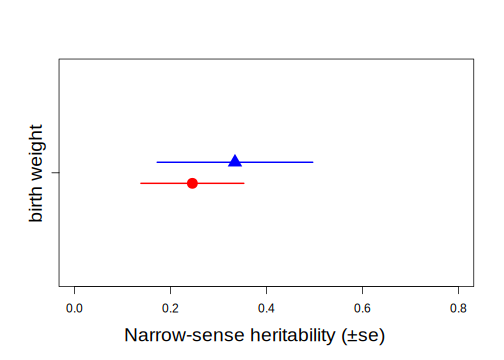
\includegraphics{wam_tuto_files/figure-latex/unnamed-chunk-27-1.pdf}
\caption{\label{fig:unnamed-chunk-27}The posterior distribution of the fixed effect (the intercept, or mean) in model 1.1}
\end{figure}

in the console, we get Figure 1 (p.~5). The plot on the left shows a time series of the values of 1000 samples of the posterior distribution of the the model intercept (mean birthweight). The plot on the right shows the same data as a distribution. Complicated statistical methods for estimating population means are of course of little interest; rather, we are examining these outputs to check that MCMCglmm's algorithms worked well for our data and for this model. The important point here is that a consistent amount of variation around a largely unchanging mean value of the intercept was obtained, and the posterior distribution of the intercept appears to be valid. More rigorous means of evaluation the independence of the samples in the posterior distribution (evaluating autocorrelation) are discussed in the MCMCglmm CourseNotes, available from CRAN. Note that your output for model 1.1 may not be identical to this due to Monte Carlo (random number) error.

The posterior distributions of the the variance components are generally of more inter- est to animal model users. We can view plots of the posterior distribution for the variance components for model 1.1 by

\begin{Shaded}
\begin{Highlighting}[]
\KeywordTok{plot}\NormalTok{(model1}\FloatTok{.1}\OperatorTok{$}\NormalTok{VCV)}
\end{Highlighting}
\end{Shaded}

\begin{figure}
\centering
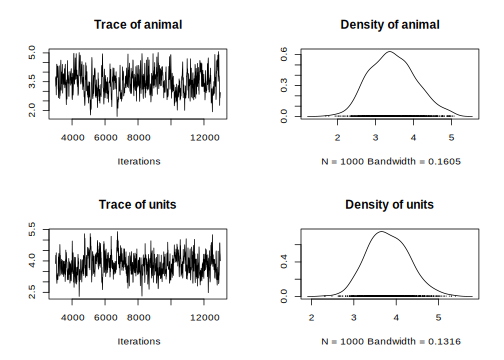
\includegraphics{wam_tuto_files/figure-latex/unnamed-chunk-28-1.pdf}
\caption{\label{fig:unnamed-chunk-28}The posterior distributions of the variance components of model 1.1, based on an analysis with the default values for nitt, burnin, and thin in MCMCglmm}
\end{figure}

which generates Figure 2 (p.~6). Here we see distributions of the estimates of the additive genetic (animal) and residual (units) effects. These samples contain some au- tocorrelation, i.e., trends are apparent in the left-hand plot. We can deal with this easily.

We will simply re-run the model for a longer number of iterations, and sample the chain less frequently. So far we have been running MCMCglmm with its default values. These defaults are a total run length of 13000 iterations, the first 3000 of which are discarded as a `burn-in' period to make sure that the converges to the part of the parameter space where the maximum likelihood exists. The remaining 10000 iterations are sampled (es- timates retained) every 10 iterations (the thinning interval). Because the values in the left-hand plots in figure 2 to appear to have different values at the beginning of the run, we might suspect that a longer burn-in period might be required. We can reduce the autocorrelation by lengthening the rest of the run and sampling the chain less frequently. The following code runs the same model 1.1, but is likely to produce better samples of the posterior distributions. This model should take about two minutes to analyze.

\begin{Shaded}
\begin{Highlighting}[]
\NormalTok{model1}\FloatTok{.1}\NormalTok{ <-}\StringTok{ }\KeywordTok{MCMCglmm}\NormalTok{(bwt }\OperatorTok{~}\StringTok{ }\DecValTok{1}\NormalTok{, }\DataTypeTok{random =} \OperatorTok{~}\NormalTok{animal, }\DataTypeTok{ginv =} \KeywordTok{list}\NormalTok{(}\DataTypeTok{animal =}\NormalTok{ Ainv), }\DataTypeTok{data =}\NormalTok{ gryphon, }\DataTypeTok{nitt =} \DecValTok{65000}\NormalTok{, }\DataTypeTok{thin =} \DecValTok{50}\NormalTok{, }\DataTypeTok{burnin =} \DecValTok{15000}\NormalTok{, }\DataTypeTok{prior =}\NormalTok{ prior1}\FloatTok{.1}\NormalTok{, }\DataTypeTok{verbose =} \OtherTok{FALSE}\NormalTok{)}
\end{Highlighting}
\end{Shaded}

Notice that we have now included the command verbose=FALSE in the MCMCglmm call. We will continue this throughout the tutorial so that more complete screen outputs can be included in this document without using too much space. Now produce the plots of the samples of the fixed and random effects (they have not been included in this document). Note that the autocorrelation is much reduced. A more compact way to evaluate the validity of the posterior distributions is to calculate autocorrelation among samples, as follows:

\begin{Shaded}
\begin{Highlighting}[]
\KeywordTok{autocorr.diag}\NormalTok{(model1}\FloatTok{.1}\OperatorTok{$}\NormalTok{VCV)}
\end{Highlighting}
\end{Shaded}

\begin{verbatim}
##                animal        units
## Lag 0     1.000000000 1.0000000000
## Lag 50    0.177204004 0.1319444721
## Lag 250  -0.008856328 0.0099887594
## Lag 500  -0.008189573 0.0059353491
## Lag 2500 -0.020351937 0.0003427092
\end{verbatim}

We will consider these levels of autocorrelation acceptable, at least for the purposes of this tutorial. Ideally, all samples of the posterior distribution should be independent, and the autocorrelation for all lag values greater than zero should be near zero. However, in practice this will not strictly be achievable for all analytical scenarios. Certainly the levels of autocorrelation observed here should not be tollerated in any formal analysis. Note that the validity of posterior distributions of any analysis should always be checked; however, for brevity we will not continue to be so consistently diligent throughout the rest of these tutorials. We can now proceed with confidence to recover some more information from these samples. We can obtain estimates of the additive genetic and residual variance by calculating the modes of the posterior distributions:

\begin{Shaded}
\begin{Highlighting}[]
\KeywordTok{posterior.mode}\NormalTok{(model1}\FloatTok{.1}\OperatorTok{$}\NormalTok{VCV)}
\end{Highlighting}
\end{Shaded}

\begin{verbatim}
##   animal    units 
## 3.199249 3.981221
\end{verbatim}

We can obtain the Bayesian equivalent of confidence intervals by calculating the the values of the estimates that bound 95\% (or any other proportion) of the posterior distri- butions:

\begin{Shaded}
\begin{Highlighting}[]
\KeywordTok{HPDinterval}\NormalTok{(model1}\FloatTok{.1}\OperatorTok{$}\NormalTok{VCV)}
\end{Highlighting}
\end{Shaded}

\begin{verbatim}
##           lower    upper
## animal 2.413592 4.733803
## units  2.784487 4.831548
## attr(,"Probability")
## [1] 0.95
\end{verbatim}

We specified weak priors in this analyses. Now we will check whether or not proper priors would have influenced the results that we obtained. The simplest way to do this is to rerun the model with different priors. Here we construct priors with a larger degree of belief parameter, and we will specify that a large proportion of the variation is under genetic control:

\begin{Shaded}
\begin{Highlighting}[]
\NormalTok{p.var <-}\StringTok{ }\KeywordTok{var}\NormalTok{(gryphon}\OperatorTok{$}\NormalTok{bwt, }\DataTypeTok{na.rm =} \OtherTok{TRUE}\NormalTok{)}
\NormalTok{prior1.}\FloatTok{1.2}\NormalTok{ <-}\StringTok{ }\KeywordTok{list}\NormalTok{(}\DataTypeTok{G =} \KeywordTok{list}\NormalTok{(}\DataTypeTok{G1 =} \KeywordTok{list}\NormalTok{(}
  \DataTypeTok{V =} \KeywordTok{matrix}\NormalTok{(p.var }\OperatorTok{*}\StringTok{ }\FloatTok{0.05}\NormalTok{),}
  \DataTypeTok{nu =} \DecValTok{1}
\NormalTok{)), }\DataTypeTok{R =} \KeywordTok{list}\NormalTok{(}\DataTypeTok{V =} \KeywordTok{matrix}\NormalTok{(p.var }\OperatorTok{*}\StringTok{ }\FloatTok{0.95}\NormalTok{), }\DataTypeTok{nu =} \DecValTok{1}\NormalTok{))}
\NormalTok{model1.}\FloatTok{1.2}\NormalTok{ <-}\StringTok{ }\KeywordTok{MCMCglmm}\NormalTok{(bwt }\OperatorTok{~}\StringTok{ }\DecValTok{1}\NormalTok{,}
  \DataTypeTok{random =} \OperatorTok{~}\NormalTok{animal, }\DataTypeTok{ginv =} \KeywordTok{list}\NormalTok{(}\DataTypeTok{animal =}\NormalTok{ Ainv),}
  \DataTypeTok{data =}\NormalTok{ gryphon, }\DataTypeTok{prior =}\NormalTok{ prior1.}\FloatTok{1.2}\NormalTok{, }\DataTypeTok{nitt =} \DecValTok{65000}\NormalTok{, }\DataTypeTok{thin =} \DecValTok{50}\NormalTok{,}
  \DataTypeTok{burnin =} \DecValTok{15000}\NormalTok{, }\DataTypeTok{verbose =} \OtherTok{FALSE}
\NormalTok{)}
\KeywordTok{posterior.mode}\NormalTok{(model1}\FloatTok{.1}\OperatorTok{$}\NormalTok{VCV)}
\end{Highlighting}
\end{Shaded}

\begin{verbatim}
##   animal    units 
## 3.199249 3.981221
\end{verbatim}

\begin{Shaded}
\begin{Highlighting}[]
\KeywordTok{posterior.mode}\NormalTok{(model1.}\FloatTok{1.2}\OperatorTok{$}\NormalTok{VCV)}
\end{Highlighting}
\end{Shaded}

\begin{verbatim}
##   animal    units 
## 3.105066 4.032622
\end{verbatim}

and we can therefore conclude that the difference in the priors has little effect on the outcome of the analysis. This is typical for an analysis where lots of data are available relative to the complexity of the model, but is often not the case. In all cases, it is important to check the effect of priors on conclusions drawn from a model.

\hypertarget{estimating-heritability-1}{%
\subsection{Estimating heritability}\label{estimating-heritability-1}}

A useful property of Bayesian posterior distributions is that we can apply almost any transformation to these distributions and they will remain valid. This applies to the calculation of heritabilities. We can obtain an estimate of the heritability by applying the basic formula h 2 =V A /V P to each sample of the posterior disribution:

\begin{Shaded}
\begin{Highlighting}[]
\NormalTok{posterior.heritability1}\FloatTok{.1}\NormalTok{ <-}\StringTok{ }\NormalTok{model1}\FloatTok{.1}\OperatorTok{$}\NormalTok{VCV[, }\StringTok{"animal"}\NormalTok{] }\OperatorTok{/}\StringTok{ }\NormalTok{(model1}\FloatTok{.1}\OperatorTok{$}\NormalTok{VCV[, }\StringTok{"animal"}\NormalTok{] }\OperatorTok{+}\StringTok{ }\NormalTok{model1}\FloatTok{.1}\OperatorTok{$}\NormalTok{VCV[, }\StringTok{"units"}\NormalTok{])}
\KeywordTok{HPDinterval}\NormalTok{(posterior.heritability1}\FloatTok{.1}\NormalTok{, }\FloatTok{0.95}\NormalTok{)}
\end{Highlighting}
\end{Shaded}

\begin{verbatim}
##          lower     upper
## var1 0.3332045 0.6110076
## attr(,"Probability")
## [1] 0.95
\end{verbatim}

\begin{Shaded}
\begin{Highlighting}[]
\KeywordTok{posterior.mode}\NormalTok{(posterior.heritability1}\FloatTok{.1}\NormalTok{)}
\end{Highlighting}
\end{Shaded}

\begin{verbatim}
##      var1 
## 0.4996456
\end{verbatim}

Generate a plot of the posterior distribution of this heritability estimate:

\begin{Shaded}
\begin{Highlighting}[]
\KeywordTok{plot}\NormalTok{(posterior.heritability1}\FloatTok{.1}\NormalTok{)}
\end{Highlighting}
\end{Shaded}

\begin{figure}
\centering
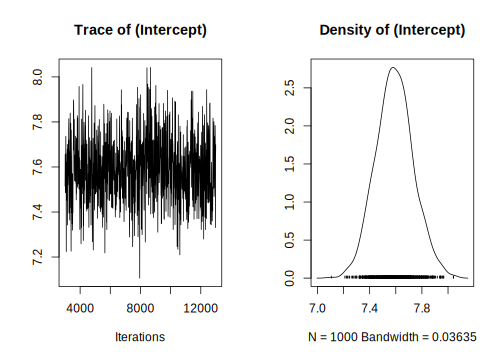
\includegraphics{wam_tuto_files/figure-latex/unnamed-chunk-35-1.pdf}
\caption{\label{fig:unnamed-chunk-35}The posterior distributions the heritability from model 1.1}
\end{figure}

\hypertarget{adding-fixed-effects-1}{%
\subsection{Adding fixed effects}\label{adding-fixed-effects-1}}

To add effects to a univariate model we simply modify the fixed effect portion of the the model specification:

\begin{Shaded}
\begin{Highlighting}[]
\NormalTok{model1}\FloatTok{.2}\NormalTok{ <-}\StringTok{ }\KeywordTok{MCMCglmm}\NormalTok{(bwt }\OperatorTok{~}\StringTok{ }\NormalTok{sex, }\DataTypeTok{random =} \OperatorTok{~}\NormalTok{animal, }\DataTypeTok{ginv =} \KeywordTok{list}\NormalTok{(}\DataTypeTok{animal =}\NormalTok{ Ainv), }\DataTypeTok{data =}\NormalTok{ gryphon, }\DataTypeTok{prior =}\NormalTok{ prior1}\FloatTok{.1}\NormalTok{, }\DataTypeTok{nitt =} \DecValTok{65000}\NormalTok{, }\DataTypeTok{thin =} \DecValTok{50}\NormalTok{, }\DataTypeTok{burnin =} \DecValTok{15000}\NormalTok{, }\DataTypeTok{verbose =} \OtherTok{FALSE}\NormalTok{)}
\end{Highlighting}
\end{Shaded}

We can assess the significance of sex as a fixed effect by examining its posterior distribution.

\begin{Shaded}
\begin{Highlighting}[]
\KeywordTok{posterior.mode}\NormalTok{(model1}\FloatTok{.2}\OperatorTok{$}\NormalTok{Sol[, }\StringTok{"sex2"}\NormalTok{])}
\end{Highlighting}
\end{Shaded}

\begin{verbatim}
##     var1 
## 2.082665
\end{verbatim}

\begin{Shaded}
\begin{Highlighting}[]
\KeywordTok{HPDinterval}\NormalTok{(model1}\FloatTok{.2}\OperatorTok{$}\NormalTok{Sol[, }\StringTok{"sex2"}\NormalTok{], }\FloatTok{0.95}\NormalTok{)}
\end{Highlighting}
\end{Shaded}

\begin{verbatim}
##         lower    upper
## var1 1.920319 2.547148
## attr(,"Probability")
## [1] 0.95
\end{verbatim}

The posterior distribution of the sex2 term does not overlap zero. Thus the we can infer that sex has a statistical effect on birthweight in this model and is a useful addition to the model, for most purposes. MCMCglmm has designated sex2 as the contrast between the two factor levels (male and female). It is also worth noting that the variance components have changed slightly:

\begin{Shaded}
\begin{Highlighting}[]
\KeywordTok{posterior.mode}\NormalTok{(model1}\FloatTok{.2}\OperatorTok{$}\NormalTok{VCV)}
\end{Highlighting}
\end{Shaded}

\begin{verbatim}
##   animal    units 
## 3.013331 3.000154
\end{verbatim}

In fact since sex effects were previously contributing to the residual variance of the model our estimate of V R (denoted 'units' in the output) is now slightly lower than before. This has an important consequence for estimating heritability since if we calculate V P as V A +V R then as we include fixed effects we will soak up more residual variance driving V P . Assuming that V A is more or less unaffected by the fixed effects fitted then as V P goes down we expect our estimate of h 2 will go up.

\begin{Shaded}
\begin{Highlighting}[]
\NormalTok{posterior.heritability1}\FloatTok{.2}\NormalTok{ <-}\StringTok{ }\NormalTok{model1}\FloatTok{.2}\OperatorTok{$}\NormalTok{VCV[, }\StringTok{"animal"}\NormalTok{] }\OperatorTok{/}\StringTok{ }\NormalTok{(model1}\FloatTok{.2}\OperatorTok{$}\NormalTok{VCV[, }\StringTok{"animal"}\NormalTok{] }\OperatorTok{+}\StringTok{ }\NormalTok{model1}\FloatTok{.2}\OperatorTok{$}\NormalTok{VCV[, }\StringTok{"units"}\NormalTok{])}
\KeywordTok{posterior.mode}\NormalTok{(posterior.heritability1}\FloatTok{.2}\NormalTok{)}
\end{Highlighting}
\end{Shaded}

\begin{verbatim}
##      var1 
## 0.4973786
\end{verbatim}

\begin{Shaded}
\begin{Highlighting}[]
\KeywordTok{HPDinterval}\NormalTok{(posterior.heritability1}\FloatTok{.2}\NormalTok{, }\FloatTok{0.95}\NormalTok{)}
\end{Highlighting}
\end{Shaded}

\begin{verbatim}
##          lower    upper
## var1 0.3790183 0.655496
## attr(,"Probability")
## [1] 0.95
\end{verbatim}

Here h 2 has increased slightly from 0.4829 to 0.5079 (again, your values may differ slightly due to Monte Carlo error). Which is the better estimate? It depends on what your question is. The first is an estimate of the proportion of variance in birth weight explained by additive effects, the latter is an estimate of the proportion of variance in birth weight after conditioning on sex that is explained by additive effects.

\hypertarget{adding-random-effects-1}{%
\subsection{Adding random effects}\label{adding-random-effects-1}}

This is done by simply modifying the model statement in the same way, but requires addition of a prior for the new random effect. For instance, we can fit an effect of birth year:

\begin{Shaded}
\begin{Highlighting}[]
\NormalTok{prior1}\FloatTok{.3}\NormalTok{ <-}\StringTok{ }\KeywordTok{list}\NormalTok{(}\DataTypeTok{G =} \KeywordTok{list}\NormalTok{(}\DataTypeTok{G1 =} \KeywordTok{list}\NormalTok{(}\DataTypeTok{V =} \DecValTok{1}\NormalTok{, }\DataTypeTok{nu =} \FloatTok{0.002}\NormalTok{), }\DataTypeTok{G2 =} \KeywordTok{list}\NormalTok{(}\DataTypeTok{V =} \DecValTok{1}\NormalTok{, }\DataTypeTok{nu =} \FloatTok{0.002}\NormalTok{)), }\DataTypeTok{R =} \KeywordTok{list}\NormalTok{(}\DataTypeTok{V =} \DecValTok{1}\NormalTok{, }\DataTypeTok{nu =} \FloatTok{0.002}\NormalTok{))}
\NormalTok{model1}\FloatTok{.3}\NormalTok{ <-}\StringTok{ }\KeywordTok{MCMCglmm}\NormalTok{(bwt }\OperatorTok{~}\StringTok{ }\NormalTok{sex, }\DataTypeTok{random =} \OperatorTok{~}\StringTok{ }\NormalTok{animal }\OperatorTok{+}\StringTok{ }\NormalTok{byear, }\DataTypeTok{ginv =} \KeywordTok{list}\NormalTok{(}\DataTypeTok{animal =}\NormalTok{ Ainv), }\DataTypeTok{data =}\NormalTok{ gryphon, }\DataTypeTok{nitt =} \DecValTok{65000}\NormalTok{, }\DataTypeTok{thin =} \DecValTok{50}\NormalTok{, }\DataTypeTok{burnin =} \DecValTok{15000}\NormalTok{, }\DataTypeTok{prior =}\NormalTok{ prior1}\FloatTok{.3}\NormalTok{, }\DataTypeTok{verbose =} \OtherTok{FALSE}\NormalTok{)}
\KeywordTok{posterior.mode}\NormalTok{(model1}\FloatTok{.3}\OperatorTok{$}\NormalTok{VCV)}
\end{Highlighting}
\end{Shaded}

\begin{verbatim}
##    animal     byear     units 
## 2.5855155 0.8071505 2.3493597
\end{verbatim}

Here the variance in birth weight explained by birth year is 0.7887. Note that although V A has changed somewhat, most of what is now partitioned as a birth year effect was previously partitioned as V R . Thus what we have really done here is to partition environ- mental effects into those arising from year to year differences versus everything else, and we do not really expect much change in h 2 (since now h 2 = V A /(V A + V BY + V R )). However, we get a somewhat different result if we also add a random effect of mother to test for maternal effects:

\begin{Shaded}
\begin{Highlighting}[]
\NormalTok{p.var <-}\StringTok{ }\KeywordTok{var}\NormalTok{(gryphon}\OperatorTok{$}\NormalTok{bwt, }\DataTypeTok{na.rm =} \OtherTok{TRUE}\NormalTok{)}
\NormalTok{prior1}\FloatTok{.4}\NormalTok{ <-}\StringTok{ }\KeywordTok{list}\NormalTok{(}\DataTypeTok{G =} \KeywordTok{list}\NormalTok{(}\DataTypeTok{G1 =} \KeywordTok{list}\NormalTok{(}\DataTypeTok{V =} \DecValTok{1}\NormalTok{, }\DataTypeTok{nu =} \FloatTok{0.002}\NormalTok{), }\DataTypeTok{G2 =} \KeywordTok{list}\NormalTok{(}
  \DataTypeTok{V =} \DecValTok{1}\NormalTok{,}
  \DataTypeTok{nu =} \FloatTok{0.002}
\NormalTok{), }\DataTypeTok{G3 =} \KeywordTok{list}\NormalTok{(}\DataTypeTok{V =} \DecValTok{1}\NormalTok{, }\DataTypeTok{nu =} \FloatTok{0.002}\NormalTok{)), }\DataTypeTok{R =} \KeywordTok{list}\NormalTok{(}
  \DataTypeTok{V =} \DecValTok{1}\NormalTok{,}
  \DataTypeTok{nu =} \FloatTok{0.002}
\NormalTok{))}
\NormalTok{model1}\FloatTok{.4}\NormalTok{ <-}\StringTok{ }\KeywordTok{MCMCglmm}\NormalTok{(bwt }\OperatorTok{~}\StringTok{ }\NormalTok{sex,}
  \DataTypeTok{random =} \OperatorTok{~}\StringTok{ }\NormalTok{animal }\OperatorTok{+}\StringTok{ }\NormalTok{byear }\OperatorTok{+}\StringTok{ }\NormalTok{mother,}
  \DataTypeTok{ginv =} \KeywordTok{list}\NormalTok{(}\DataTypeTok{animal =}\NormalTok{ Ainv), }\DataTypeTok{data =}\NormalTok{ gryphon, }\DataTypeTok{nitt =} \DecValTok{65000}\NormalTok{, }\DataTypeTok{thin =} \DecValTok{50}\NormalTok{, }\DataTypeTok{burnin =} \DecValTok{15000}\NormalTok{,}
  \DataTypeTok{prior =}\NormalTok{ prior1}\FloatTok{.4}\NormalTok{, }\DataTypeTok{verbose =} \OtherTok{FALSE}
\NormalTok{)}
\KeywordTok{posterior.mode}\NormalTok{(model1}\FloatTok{.4}\OperatorTok{$}\NormalTok{VCV)}
\end{Highlighting}
\end{Shaded}

\begin{verbatim}
##   animal    byear   mother    units 
## 2.401821 0.793273 1.145345 1.605242
\end{verbatim}

Here partitioning of significant maternal variance has resulted in a further decrease in V R but also a decrease in V A . The latter is because maternal effects of the sort we simulated (fixed differences between mothers) will have the consequence of increasing similarity among maternal siblings. Consequently they can look very much like additive genetic effects and if present, but unmodelled, represent a type of `common environment effect' that can - and will- cause upward bias in V A and so h 2 . Let's compare the estimates of heritability from each of models 1.2, 1.3 and 1.4:

\begin{Shaded}
\begin{Highlighting}[]
\NormalTok{posterior.heritability1}\FloatTok{.3}\NormalTok{ <-}\StringTok{ }\NormalTok{model1}\FloatTok{.3}\OperatorTok{$}\NormalTok{VCV[, }\StringTok{"animal"}\NormalTok{] }\OperatorTok{/}\StringTok{ }\NormalTok{(model1}\FloatTok{.3}\OperatorTok{$}\NormalTok{VCV[, }\StringTok{"animal"}\NormalTok{] }\OperatorTok{+}\StringTok{ }\NormalTok{model1}\FloatTok{.3}\OperatorTok{$}\NormalTok{VCV[, }\StringTok{"byear"}\NormalTok{] }\OperatorTok{+}\StringTok{ }\NormalTok{model1}\FloatTok{.3}\OperatorTok{$}\NormalTok{VCV[, }\StringTok{"units"}\NormalTok{])}
\NormalTok{posterior.heritability1}\FloatTok{.4}\NormalTok{ <-}\StringTok{ }\NormalTok{model1}\FloatTok{.4}\OperatorTok{$}\NormalTok{VCV[, }\StringTok{"animal"}\NormalTok{] }\OperatorTok{/}\StringTok{ }\NormalTok{(model1}\FloatTok{.4}\OperatorTok{$}\NormalTok{VCV[, }\StringTok{"animal"}\NormalTok{] }\OperatorTok{+}\StringTok{ }\NormalTok{model1}\FloatTok{.4}\OperatorTok{$}\NormalTok{VCV[, }\StringTok{"byear"}\NormalTok{] }\OperatorTok{+}\StringTok{ }\NormalTok{model1}\FloatTok{.4}\OperatorTok{$}\NormalTok{VCV[, }\StringTok{"mother"}\NormalTok{] }\OperatorTok{+}\StringTok{ }\NormalTok{model1}\FloatTok{.4}\OperatorTok{$}\NormalTok{VCV[, }\StringTok{"units"}\NormalTok{])}
\KeywordTok{posterior.mode}\NormalTok{(posterior.heritability1}\FloatTok{.2}\NormalTok{)}
\end{Highlighting}
\end{Shaded}

\begin{verbatim}
##      var1 
## 0.4973786
\end{verbatim}

\begin{Shaded}
\begin{Highlighting}[]
\KeywordTok{posterior.mode}\NormalTok{(posterior.heritability1}\FloatTok{.3}\NormalTok{)}
\end{Highlighting}
\end{Shaded}

\begin{verbatim}
##      var1 
## 0.4477868
\end{verbatim}

\begin{Shaded}
\begin{Highlighting}[]
\KeywordTok{posterior.mode}\NormalTok{(posterior.heritability1}\FloatTok{.4}\NormalTok{)}
\end{Highlighting}
\end{Shaded}

\begin{verbatim}
##      var1 
## 0.4027288
\end{verbatim}

\hypertarget{testing-significance-of-variance-components}{%
\subsection{Testing significance of variance components}\label{testing-significance-of-variance-components}}

While testing the significance of fixed effects by evaluating whether or not their posterior distributions overlap zero was simple and valid, this approach does not work for vari- ance components. Variance components are bound to be positive (given a proper prior), and thus even when a random effect is not meaningful, its posterior distribution will never overlap zero. Model comparisons can be performed using the deviance information criterion (DIC), although it should be noted that the properties of DIC are not well un- derstood and that the DIC may be focused at the wrong level for most people's intended level of infernce - particularly with non-Gaussian responses. The implementation of DIC in MCMCglmm is further described in the reference manual. DIC values are calculated by MCMCglmm by default. Briefly, DIC like other information criteria balance model fit and model complexity simultaneously, and small values of DIC are prefered. We can compare models 1.4 and 1.3, i.e., models with and without the mother term:

\begin{Shaded}
\begin{Highlighting}[]
\NormalTok{model1}\FloatTok{.3}\OperatorTok{$}\NormalTok{DIC}
\end{Highlighting}
\end{Shaded}

\begin{verbatim}
## [1] 3550.392
\end{verbatim}

\begin{Shaded}
\begin{Highlighting}[]
\NormalTok{model1}\FloatTok{.4}\OperatorTok{$}\NormalTok{DIC}
\end{Highlighting}
\end{Shaded}

\begin{verbatim}
## [1] 3314.328
\end{verbatim}

model 1.4 has a much lower DIC value. Since the maternal effect term is the only difference between the models, we can consider the inclusion of this term statistically justifiable. We should note however that DIC has a large sampling variance and should probably only be calculated based on much longer MCMC runs.

\hypertarget{brms-1}{%
\section{brms}\label{brms-1}}

\begin{Shaded}
\begin{Highlighting}[]
\KeywordTok{library}\NormalTok{(brms)}
\NormalTok{Amat <-}\StringTok{ }\KeywordTok{as.matrix}\NormalTok{(nadiv}\OperatorTok{::}\KeywordTok{makeA}\NormalTok{(gryphonped))}
\NormalTok{brms_m1}\FloatTok{.1}\NormalTok{ <-}\StringTok{ }\KeywordTok{brm}\NormalTok{(}
\NormalTok{  bwt }\OperatorTok{~}\StringTok{ }\DecValTok{1} \OperatorTok{+}\StringTok{ }\NormalTok{(}\DecValTok{1} \OperatorTok{|}\StringTok{ }\KeywordTok{gr}\NormalTok{(animal, }\DataTypeTok{cov =}\NormalTok{ Amat)),}
  \DataTypeTok{data =}\NormalTok{ gryphon,}
  \DataTypeTok{data2 =} \KeywordTok{list}\NormalTok{(}\DataTypeTok{Amat =}\NormalTok{ Amat),}
  \DataTypeTok{family =} \KeywordTok{gaussian}\NormalTok{(),}
  \DataTypeTok{chains =} \DecValTok{2}\NormalTok{, }\DataTypeTok{cores =} \DecValTok{2}\NormalTok{, }\DataTypeTok{iter =} \DecValTok{1000}
\NormalTok{)}
\KeywordTok{save}\NormalTok{(brms_m1}\FloatTok{.1}\NormalTok{, }\DataTypeTok{file =} \StringTok{"data/brms_m1_1.rda"}\NormalTok{)}
\end{Highlighting}
\end{Shaded}

\begin{Shaded}
\begin{Highlighting}[]
\KeywordTok{load}\NormalTok{(}\StringTok{"data/brms_m1_1.rda"}\NormalTok{)}
\KeywordTok{summary}\NormalTok{(brms_m1}\FloatTok{.1}\NormalTok{)}
\end{Highlighting}
\end{Shaded}

\begin{verbatim}
##  Family: gaussian 
##   Links: mu = identity; sigma = identity 
## Formula: bwt ~ 1 + (1 | gr(animal, cov = Amat)) 
##    Data: gryphon (Number of observations: 854) 
## Samples: 2 chains, each with iter = 1000; warmup = 500; thin = 1;
##          total post-warmup samples = 1000
## 
## Group-Level Effects: 
## ~animal (Number of levels: 854) 
##               Estimate Est.Error l-95% CI u-95% CI Rhat Bulk_ESS Tail_ESS
## sd(Intercept)     1.83      0.17     1.47     2.15 1.04       60      224
## 
## Population-Level Effects: 
##           Estimate Est.Error l-95% CI u-95% CI Rhat Bulk_ESS Tail_ESS
## Intercept     7.58      0.15     7.29     7.88 1.00      639      558
## 
## Family Specific Parameters: 
##       Estimate Est.Error l-95% CI u-95% CI Rhat Bulk_ESS Tail_ESS
## sigma     1.96      0.13     1.71     2.22 1.04       57      165
## 
## Samples were drawn using sampling(NUTS). For each parameter, Bulk_ESS
## and Tail_ESS are effective sample size measures, and Rhat is the potential
## scale reduction factor on split chains (at convergence, Rhat = 1).
\end{verbatim}

\begin{Shaded}
\begin{Highlighting}[]
\KeywordTok{plot}\NormalTok{(brms_m1}\FloatTok{.1}\NormalTok{)}
\end{Highlighting}
\end{Shaded}

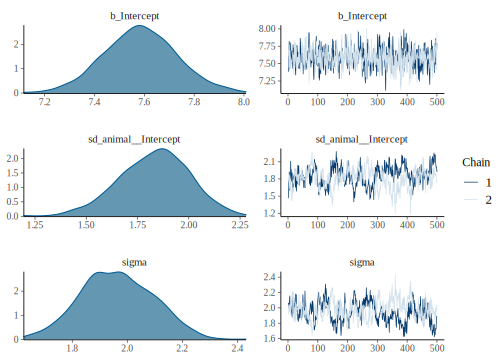
\includegraphics{wam_tuto_files/figure-latex/unnamed-chunk-45-1.pdf}

\hypertarget{multivariate-animal-model}{%
\chapter{Multivariate animal model}\label{multivariate-animal-model}}

This tutorial will demonstrate how to run a multivariate animal model looking at birth weight and tarsus length of the phenomenal gryphons.

\hypertarget{scenario-and-data-1}{%
\section{Scenario and data}\label{scenario-and-data-1}}

\hypertarget{scenario-1}{%
\subsection{Scenario}\label{scenario-1}}

Since natural selection rarely acts on single traits, to understand how birth weight might evolve in our population of gryphons, we may also want to think about possible covariance with other traits. If tarsus length at fledging is also under positive selection, what implications does this have for birth weight and vice versa? If the two traits are positively genetically correlated then this will facilitate evolution of larger size (since response of one trait will induce a positively correlated response in the other). If there is negative genetic covariance then this could act as an evolutionary constraint.

Using multivariate models allows the estimation of parameters relating to each trait alone (\emph{i.e.} \(V_A\), \(h^2\), etc), but also yields estimates of covariance components between traits. These include the (additive) genetic covariance \(COV_A\) which is often rescaled to give the additive genetic correlation \(r_A\). However, covariance can also arise through other random effects (\emph{e.g.} maternal covariance) and these sources can also be explicitly modelled in a bivariate analysis.

\hypertarget{gryphon-files}{%
\subsection{gryphon files}\label{gryphon-files}}

gryphonpedigree and phenotypic data files are the same as those used in tutorial 1 (\emph{i.e}, \texttt{gryphonped.csv} and \texttt{gryphon.csv} respectively).

Reading the data

\begin{Shaded}
\begin{Highlighting}[]
\NormalTok{gryphon <-}\StringTok{ }\KeywordTok{read.csv}\NormalTok{(}\StringTok{"data/gryphon.csv"}\NormalTok{)}
\NormalTok{gryphon}\OperatorTok{$}\NormalTok{animal <-}\StringTok{ }\KeywordTok{as.factor}\NormalTok{(gryphon}\OperatorTok{$}\NormalTok{animal)}
\NormalTok{gryphon}\OperatorTok{$}\NormalTok{mother <-}\StringTok{ }\KeywordTok{as.factor}\NormalTok{(gryphon}\OperatorTok{$}\NormalTok{mother)}
\NormalTok{gryphon}\OperatorTok{$}\NormalTok{byear <-}\StringTok{ }\KeywordTok{as.factor}\NormalTok{(gryphon}\OperatorTok{$}\NormalTok{byear)}
\NormalTok{gryphon}\OperatorTok{$}\NormalTok{sex <-}\StringTok{ }\KeywordTok{as.factor}\NormalTok{(gryphon}\OperatorTok{$}\NormalTok{sex)}
\NormalTok{gryphon}\OperatorTok{$}\NormalTok{bwt <-}\StringTok{ }\KeywordTok{as.numeric}\NormalTok{(gryphon}\OperatorTok{$}\NormalTok{bwt)}
\NormalTok{gryphon}\OperatorTok{$}\NormalTok{tarsus <-}\StringTok{ }\KeywordTok{as.numeric}\NormalTok{(gryphon}\OperatorTok{$}\NormalTok{tarsus)}
\end{Highlighting}
\end{Shaded}

Reading the pedigree

\begin{Shaded}
\begin{Highlighting}[]
\NormalTok{gryphonped <-}\StringTok{ }\KeywordTok{read.csv}\NormalTok{(}\StringTok{"data/gryphonped.csv"}\NormalTok{)}
\NormalTok{gryphonped}\OperatorTok{$}\NormalTok{id <-}\StringTok{ }\KeywordTok{as.factor}\NormalTok{(gryphonped}\OperatorTok{$}\NormalTok{id)}
\NormalTok{gryphonped}\OperatorTok{$}\NormalTok{father <-}\StringTok{ }\KeywordTok{as.factor}\NormalTok{(gryphonped}\OperatorTok{$}\NormalTok{father)}
\NormalTok{gryphonped}\OperatorTok{$}\NormalTok{mother <-}\StringTok{ }\KeywordTok{as.factor}\NormalTok{(gryphonped}\OperatorTok{$}\NormalTok{mother)}
\end{Highlighting}
\end{Shaded}

\hypertarget{asreml-biv}{%
\section{Asreml-R}\label{asreml-biv}}

\hypertarget{running-the-model-2}{%
\subsection{Running the model}\label{running-the-model-2}}

For running multivariate analyses in ASReml-R, the code is slightly more complex than for the univariate case. This is because ASReml-R allows us to make different assumptions about the way in which traits might be related and so we need to explicitly code a model of the (co)variance structure we want to fit. We have also specified some starting values. These are can be very approximate \emph{guestimates}, but having reasonable starting values can aid convergence. Finally, we have increased the default maximum number of iterations (\texttt{maxiter}) which can help to achieve convergence for more complicated models.

\begin{Shaded}
\begin{Highlighting}[]
\NormalTok{ainv <-}\StringTok{ }\KeywordTok{ainverse}\NormalTok{(gryphonped)}
\NormalTok{modela <-}\StringTok{ }\KeywordTok{asreml}\NormalTok{(}
  \DataTypeTok{fixed =} \KeywordTok{cbind}\NormalTok{(bwt, tarsus) }\OperatorTok{~}\StringTok{ }\NormalTok{trait,}
  \DataTypeTok{random =} \OperatorTok{~}\StringTok{ }\KeywordTok{us}\NormalTok{(trait)}\OperatorTok{:}\KeywordTok{vm}\NormalTok{(animal, ainv), }\DataTypeTok{init =} \KeywordTok{c}\NormalTok{(}\DecValTok{1}\NormalTok{, }\FloatTok{0.1}\NormalTok{, }\DecValTok{1}\NormalTok{),}
  \DataTypeTok{residual =} \OperatorTok{~}\StringTok{ }\KeywordTok{id}\NormalTok{(units)}\OperatorTok{:}\KeywordTok{us}\NormalTok{(trait, }\DataTypeTok{init =} \KeywordTok{c}\NormalTok{(}\DecValTok{1}\NormalTok{, }\FloatTok{0.1}\NormalTok{, }\DecValTok{1}\NormalTok{)),}
  \DataTypeTok{data =}\NormalTok{ gryphon,}
  \DataTypeTok{maxit =} \DecValTok{20}
\NormalTok{)}
\end{Highlighting}
\end{Shaded}

\begin{verbatim}
## Model fitted using the sigma parameterization.
## ASReml 4.1.0 Fri Feb 12 17:19:47 2021
##           LogLik        Sigma2     DF     wall    cpu
##  1     -5118.122           1.0   1535 17:19:47    0.0
##  2     -4358.769           1.0   1535 17:19:47    0.0
##  3     -3540.792           1.0   1535 17:19:47    0.0
##  4     -3004.970           1.0   1535 17:19:47    0.0
##  5     -2747.831           1.0   1535 17:19:47    0.0
##  6     -2687.807           1.0   1535 17:19:47    0.0
##  7     -2680.057           1.0   1535 17:19:47    0.0
##  8     -2679.743           1.0   1535 17:19:47    0.0
##  9     -2679.741           1.0   1535 17:19:47    0.0
\end{verbatim}

This has fitted a bivariate model of \texttt{bwt} and \texttt{tarsus}, with the mean for each of the traits as a fixed effect (\texttt{trait}). The additive genetic variance-covariance matrix (\(\textbf{G}\)) is unstructured (\texttt{us}; \emph{i.e.} all elements are free to vary) and the starting values for \(V_A\) for \texttt{bwt}, \(COV_A\) between \texttt{bwt} and \texttt{tarsus}, and \(V_A\) for \texttt{tarsus} are set to 1, 0.1 and 1, respectively. Similarly, the residual matrix is unstructured and uses the same starting values.

Let's have a look at the variance components, and notice that there are now six (co)variance components reported in the table:

\begin{Shaded}
\begin{Highlighting}[]
\KeywordTok{summary}\NormalTok{(modela)}\OperatorTok{$}\NormalTok{varcomp}
\end{Highlighting}
\end{Shaded}

\begin{verbatim}
##                                            component std.error  z.ratio bound
## trait:vm(animal, ainv)!trait_bwt:bwt        3.368498 0.6349441 5.305188     P
## trait:vm(animal, ainv)!trait_tarsus:bwt     2.460195 1.0735865 2.291567     P
## trait:vm(animal, ainv)!trait_tarsus:tarsus 12.346837 3.0753775 4.014739     P
## units:trait!R                               1.000000        NA       NA     F
## units:trait!trait_bwt:bwt                   3.849836 0.5199897 7.403677     P
## units:trait!trait_tarsus:bwt                3.312978 0.9128834 3.629136     P
## units:trait!trait_tarsus:tarsus            17.645584 2.6668492 6.616641     P
##                                            %ch
## trait:vm(animal, ainv)!trait_bwt:bwt       0.0
## trait:vm(animal, ainv)!trait_tarsus:bwt    0.2
## trait:vm(animal, ainv)!trait_tarsus:tarsus 0.1
## units:trait!R                              0.0
## units:trait!trait_bwt:bwt                  0.0
## units:trait!trait_tarsus:bwt               0.1
## units:trait!trait_tarsus:tarsus            0.1
\end{verbatim}

The first three terms relate to the genetic matrix and, in order are \(V_{A,bwt}\), \(COV_A\), \(V_{A, tarsus}\). Below is again a line where the \texttt{units:traitr!R} component equals 1, which again can be ignored. The final three terms relate to the residual matrix and correspond to \(V_{R,bwt}\), \(COV_R\), \(V_{R,tarsus}\). Based on our quick and dirty check (is \texttt{z.ratio} \textgreater{} 1.96?) all components look to be statistically significant.

We can calculate the genetic correlation as \(COV_A / \sqrt{V_{A,bwt} \cdot V_{A,tarsus}}\). Thus this model gives an estimate of \(r_A\) = 0.38. Although we can calculate this by hand, we can also use \texttt{vpredict()}, which also provides an (approximate) standard error:

\begin{Shaded}
\begin{Highlighting}[]
\KeywordTok{vpredict}\NormalTok{(modela, rA }\OperatorTok{~}\StringTok{ }\NormalTok{V2 }\OperatorTok{/}\StringTok{ }\KeywordTok{sqrt}\NormalTok{(V1 }\OperatorTok{*}\StringTok{ }\NormalTok{V3))}
\end{Highlighting}
\end{Shaded}

\begin{verbatim}
##     Estimate       SE
## rA 0.3814816 0.129991
\end{verbatim}

Of course we can also calculate the heritability of \texttt{bwt} and \texttt{tarsus} from this model:

\begin{Shaded}
\begin{Highlighting}[]
\KeywordTok{vpredict}\NormalTok{(modela, h2.bwt }\OperatorTok{~}\StringTok{ }\NormalTok{V1 }\OperatorTok{/}\StringTok{ }\NormalTok{(V1 }\OperatorTok{+}\StringTok{ }\NormalTok{V5))}
\end{Highlighting}
\end{Shaded}

\begin{verbatim}
##         Estimate         SE
## h2.bwt 0.4666586 0.07672219
\end{verbatim}

\begin{Shaded}
\begin{Highlighting}[]
\KeywordTok{vpredict}\NormalTok{(modela, h2.tarsus }\OperatorTok{~}\StringTok{ }\NormalTok{V3 }\OperatorTok{/}\StringTok{ }\NormalTok{(V3 }\OperatorTok{+}\StringTok{ }\NormalTok{V7))}
\end{Highlighting}
\end{Shaded}

\begin{verbatim}
##            Estimate        SE
## h2.tarsus 0.4116652 0.0930738
\end{verbatim}

\hypertarget{adding-fixed-and-random-effects}{%
\subsection{Adding fixed and random effects}\label{adding-fixed-and-random-effects}}

Fixed and random effects can be added just as for the univariate case. Given that our full model of bwt from tutorial 1 had sex as a fixed effect as well as random effects of birth year and mother we could specify a bivariate formulation of this using:

\begin{Shaded}
\begin{Highlighting}[]
\NormalTok{modelb <-}\StringTok{ }\KeywordTok{asreml}\NormalTok{(}
  \DataTypeTok{fixed =} \KeywordTok{cbind}\NormalTok{(bwt, tarsus) }\OperatorTok{~}\StringTok{ }\NormalTok{trait }\OperatorTok{+}\StringTok{ }\NormalTok{trait}\OperatorTok{:}\NormalTok{sex,}
  \DataTypeTok{random =} \OperatorTok{~}\StringTok{ }\KeywordTok{us}\NormalTok{(trait, }\DataTypeTok{init =} \KeywordTok{c}\NormalTok{(}\DecValTok{1}\NormalTok{, }\FloatTok{0.1}\NormalTok{, }\DecValTok{1}\NormalTok{))}\OperatorTok{:}\KeywordTok{vm}\NormalTok{(animal, ainv) }\OperatorTok{+}
\StringTok{    }\KeywordTok{us}\NormalTok{(trait, }\DataTypeTok{init =} \KeywordTok{c}\NormalTok{(}\DecValTok{1}\NormalTok{, }\FloatTok{0.1}\NormalTok{, }\DecValTok{1}\NormalTok{))}\OperatorTok{:}\NormalTok{byear }\OperatorTok{+}
\StringTok{    }\KeywordTok{us}\NormalTok{(trait, }\DataTypeTok{init =} \KeywordTok{c}\NormalTok{(}\DecValTok{1}\NormalTok{, }\FloatTok{0.1}\NormalTok{, }\DecValTok{1}\NormalTok{))}\OperatorTok{:}\NormalTok{mother,}
  \DataTypeTok{residual =} \OperatorTok{~}\StringTok{ }\KeywordTok{id}\NormalTok{(units)}\OperatorTok{:}\KeywordTok{us}\NormalTok{(trait, }\DataTypeTok{init =} \KeywordTok{c}\NormalTok{(}\DecValTok{1}\NormalTok{, }\FloatTok{0.1}\NormalTok{, }\DecValTok{1}\NormalTok{)),}
  \DataTypeTok{data =}\NormalTok{ gryphon,}
  \DataTypeTok{maxit =} \DecValTok{20}
\NormalTok{)}
\end{Highlighting}
\end{Shaded}

\begin{verbatim}
## Model fitted using the sigma parameterization.
## ASReml 4.1.0 Fri Feb 12 17:19:47 2021
##           LogLik        Sigma2     DF     wall    cpu
##  1     -4672.301           1.0   1533 17:19:47    0.0
##  2     -4005.615           1.0   1533 17:19:47    0.0
##  3     -3271.483           1.0   1533 17:19:47    0.0 (1 restrained)
##  4     -2761.414           1.0   1533 17:19:47    0.0 (1 restrained)
##  5     -2481.356           1.0   1533 17:19:47    0.0
##  6     -2395.858           1.0   1533 17:19:47    0.0
##  7     -2381.050           1.0   1533 17:19:47    0.0
##  8     -2380.251           1.0   1533 17:19:47    0.0
##  9     -2380.246           1.0   1533 17:19:47    0.0
\end{verbatim}

Note that we have specified a covariance structure for each random effect and an estimate of the effect of sex on both birth weight and tarsus length by interacting sex with trait in the fixed effect structure.

There will now be twelve (co)variance components reported after running the code:

\begin{Shaded}
\begin{Highlighting}[]
\KeywordTok{summary}\NormalTok{(modelb)}\OperatorTok{$}\NormalTok{varcomp}
\end{Highlighting}
\end{Shaded}

\begin{verbatim}
##                                             component std.error    z.ratio
## trait:byear!trait_bwt:bwt                   0.9746500 0.2825643  3.4493030
## trait:byear!trait_tarsus:bwt                0.1624455 0.4185658  0.3881003
## trait:byear!trait_tarsus:tarsus             3.7384670 1.2069893  3.0973489
## trait:mother!trait_bwt:bwt                  1.1445030 0.2302062  4.9716424
## trait:mother!trait_tarsus:bwt              -1.5566953 0.4051695 -3.8420841
## trait:mother!trait_tarsus:tarsus            4.8206658 1.3200970  3.6517512
## trait:vm(animal, ainv)!trait_bwt:bwt        1.9893623 0.4410265  4.5107542
## trait:vm(animal, ainv)!trait_tarsus:bwt     3.3168101 0.9030192  3.6730229
## trait:vm(animal, ainv)!trait_tarsus:tarsus 10.2277887 2.8065673  3.6442343
## units:trait!R                               1.0000000        NA         NA
## units:trait!trait_bwt:bwt                   1.8443114 0.3443161  5.3564488
## units:trait!trait_tarsus:bwt                4.0144042 0.7411868  5.4161844
## units:trait!trait_tarsus:tarsus            12.4857174 2.2890289  5.4545915
##                                            bound %ch
## trait:byear!trait_bwt:bwt                      P 0.0
## trait:byear!trait_tarsus:bwt                   P 0.0
## trait:byear!trait_tarsus:tarsus                P 0.0
## trait:mother!trait_bwt:bwt                     P 0.0
## trait:mother!trait_tarsus:bwt                  P 0.0
## trait:mother!trait_tarsus:tarsus               P 0.0
## trait:vm(animal, ainv)!trait_bwt:bwt           P 0.0
## trait:vm(animal, ainv)!trait_tarsus:bwt        P 0.1
## trait:vm(animal, ainv)!trait_tarsus:tarsus     P 0.1
## units:trait!R                                  F 0.0
## units:trait!trait_bwt:bwt                      P 0.0
## units:trait!trait_tarsus:bwt                   P 0.0
## units:trait!trait_tarsus:tarsus                P 0.1
\end{verbatim}

\hypertarget{significance-testing}{%
\subsection{Significance testing}\label{significance-testing}}

Under the model above \(r_M\) is estimated as -0.66 and the \texttt{z.ratio} associated with the corresponding covariance (\(COV_M\)) is \textgreater{}2 (in absolute terms). We might therefore infer that there is evidence for a strong negative correlation between the traits with respect to the mother and that while maternal identity explains variance in both traits those mothers that tend to produce heavier offspring actually tend to produce offspring with shorter tarsus lengths.

To formally test if \(COV_M\) is significantly different from zero, we can compare the log-likelihood for this model:

\begin{Shaded}
\begin{Highlighting}[]
\NormalTok{modelb}\OperatorTok{$}\NormalTok{loglik}
\end{Highlighting}
\end{Shaded}

\begin{verbatim}
## [1] -2380.246
\end{verbatim}

to a model in which we specify that \(COV_M\)=0. Since this constraint reduces the number of parameters to be estimated by one, we can use a likelihood ratio test with one degree of freedom. To run the constrained model, we modify the G structure definition for the \texttt{mother} random effect to diagonal (\texttt{diag}), which means we only estimate the variances (the diagonal of the matrix) but not the covariance:

\begin{Shaded}
\begin{Highlighting}[]
\NormalTok{modelc <-}\StringTok{ }\KeywordTok{asreml}\NormalTok{(}
  \DataTypeTok{fixed =} \KeywordTok{cbind}\NormalTok{(bwt, tarsus) }\OperatorTok{~}\StringTok{ }\NormalTok{trait }\OperatorTok{+}\StringTok{ }\NormalTok{trait}\OperatorTok{:}\NormalTok{sex,}
  \DataTypeTok{random =} \OperatorTok{~}\StringTok{ }\KeywordTok{us}\NormalTok{(trait, }\DataTypeTok{init =} \KeywordTok{c}\NormalTok{(}\DecValTok{1}\NormalTok{, }\FloatTok{0.1}\NormalTok{, }\DecValTok{1}\NormalTok{))}\OperatorTok{:}\KeywordTok{vm}\NormalTok{(animal, ainv) }\OperatorTok{+}
\StringTok{    }\KeywordTok{us}\NormalTok{(trait, }\DataTypeTok{init =} \KeywordTok{c}\NormalTok{(}\DecValTok{1}\NormalTok{, }\FloatTok{0.1}\NormalTok{, }\DecValTok{1}\NormalTok{))}\OperatorTok{:}\NormalTok{byear }\OperatorTok{+}
\StringTok{    }\KeywordTok{diag}\NormalTok{(trait, }\DataTypeTok{init =} \KeywordTok{c}\NormalTok{(}\DecValTok{1}\NormalTok{, }\DecValTok{1}\NormalTok{))}\OperatorTok{:}\NormalTok{mother,}
  \DataTypeTok{residual =} \OperatorTok{~}\StringTok{ }\KeywordTok{id}\NormalTok{(units)}\OperatorTok{:}\KeywordTok{us}\NormalTok{(trait, }\DataTypeTok{init =} \KeywordTok{c}\NormalTok{(}\DecValTok{1}\NormalTok{, }\FloatTok{0.1}\NormalTok{, }\DecValTok{1}\NormalTok{)),}
  \DataTypeTok{data =}\NormalTok{ gryphon,}
  \DataTypeTok{maxit =} \DecValTok{20}
\NormalTok{)}
\end{Highlighting}
\end{Shaded}

\begin{verbatim}
## Model fitted using the sigma parameterization.
## ASReml 4.1.0 Fri Feb 12 17:19:48 2021
##           LogLik        Sigma2     DF     wall    cpu
##  1     -4677.820           1.0   1533 17:19:48    0.1
##  2     -4010.442           1.0   1533 17:19:48    0.0
##  3     -3275.409           1.0   1533 17:19:48    0.0
##  4     -2763.519           1.0   1533 17:19:48    0.0
##  5     -2483.732           1.0   1533 17:19:48    0.0
##  6     -2400.242           1.0   1533 17:19:48    0.0
##  7     -2386.663           1.0   1533 17:19:48    0.0
##  8     -2386.049           1.0   1533 17:19:48    0.0
##  9     -2386.045           1.0   1533 17:19:48    0.0
\end{verbatim}

You can run \texttt{summary(modelc)\$varcomp} to confirm this worked. We can now obtain the log-likelihood of this model and compare this to that of \texttt{modelb} using a likelihood ratio test:

\begin{Shaded}
\begin{Highlighting}[]
\NormalTok{modelc}\OperatorTok{$}\NormalTok{loglik}
\end{Highlighting}
\end{Shaded}

\begin{verbatim}
## [1] -2386.045
\end{verbatim}

We can see that the model log-likelihood is now -2386.05.
And comparing the models using a likelihood ratio test:

\begin{Shaded}
\begin{Highlighting}[]
\DecValTok{2} \OperatorTok{*}\StringTok{ }\NormalTok{(modelb}\OperatorTok{$}\NormalTok{loglik }\OperatorTok{-}\StringTok{ }\NormalTok{modelc}\OperatorTok{$}\NormalTok{loglik)}
\end{Highlighting}
\end{Shaded}

\begin{verbatim}
## [1] 11.59831
\end{verbatim}

So our chi-square test statistic is \(\chi^2_1\)= 11.6.
The p-value that goes with this is obtained by:

\begin{Shaded}
\begin{Highlighting}[]
\DecValTok{1} \OperatorTok{-}\StringTok{ }\KeywordTok{pchisq}\NormalTok{(}\DecValTok{2} \OperatorTok{*}\StringTok{ }\NormalTok{(modelb}\OperatorTok{$}\NormalTok{loglik }\OperatorTok{-}\StringTok{ }\NormalTok{modelc}\OperatorTok{$}\NormalTok{loglik), }\DecValTok{1}\NormalTok{)}
\end{Highlighting}
\end{Shaded}

\begin{verbatim}
## [1] 0.000660117
\end{verbatim}

We would therefore conclude that the maternal covariance is significantly different from zero.

We could apply the same procedure to show that the residual (environmental) covariance and the genetic covariance estimates are significantly greater than zero (\emph{i.e.}, heavier individuals tend to have longer tarsus lengths). In contrast, we should find that the byear covariance between the two traits is non-significant.

\hypertarget{gremlin-2}{%
\section{gremlin}\label{gremlin-2}}

Not implemented yet

\hypertarget{mcmcglmm-2}{%
\section{MCMCglmm}\label{mcmcglmm-2}}

All others software will remove automatically lines with missing data from the dataset use to fit the model.
\texttt{MCMCglmm}, however, will not do it and will try to fit the model use latent variables for missing data.
For comparison, we will remove the missing values from the data before fitting the model.

\begin{Shaded}
\begin{Highlighting}[]
\NormalTok{gryphon <-}\StringTok{ }\KeywordTok{subset}\NormalTok{(gryphon, }\OperatorTok{!}\KeywordTok{is.na}\NormalTok{(bwt) }\OperatorTok{&}\StringTok{ }\OperatorTok{!}\KeywordTok{is.na}\NormalTok{(tarsus))}
\end{Highlighting}
\end{Shaded}

\hypertarget{fitting-the-model}{%
\subsection{Fitting the model}\label{fitting-the-model}}

Fitting a multivariate model in MCMCglmm involves several new consideration above those for fitting univariate models. First, we have to fit multivariate priors; second, we have to specify the ways in which effects on different traits may covary, including the nature of residual (co)variation; and third, we will have to be a little more specific when specifying to MCMCglmm what type of distributions from which we assume our data are drawn. Our most basic model can be specified as:

\begin{Shaded}
\begin{Highlighting}[]
\KeywordTok{library}\NormalTok{(MCMCglmm)}
\NormalTok{Ainv <-}\StringTok{ }\KeywordTok{inverseA}\NormalTok{(gryphonped)}\OperatorTok{$}\NormalTok{Ainv}
\NormalTok{prior2}\FloatTok{.1}\NormalTok{ <-}\StringTok{ }\KeywordTok{list}\NormalTok{(}
  \DataTypeTok{G =} \KeywordTok{list}\NormalTok{(}\DataTypeTok{G1 =} \KeywordTok{list}\NormalTok{(}\DataTypeTok{V =} \KeywordTok{diag}\NormalTok{(}\DecValTok{2}\NormalTok{), }\DataTypeTok{nu =} \FloatTok{1.002}\NormalTok{)),}
  \DataTypeTok{R =} \KeywordTok{list}\NormalTok{(}\DataTypeTok{V =} \KeywordTok{diag}\NormalTok{(}\DecValTok{2}\NormalTok{), }\DataTypeTok{nu =} \FloatTok{1.002}\NormalTok{)}
\NormalTok{)}
\NormalTok{model2}\FloatTok{.1}\NormalTok{ <-}\StringTok{ }\KeywordTok{MCMCglmm}\NormalTok{(}\KeywordTok{cbind}\NormalTok{(bwt, tarsus) }\OperatorTok{~}\StringTok{ }\NormalTok{trait }\OperatorTok{-}\StringTok{ }\DecValTok{1}\NormalTok{,}
  \DataTypeTok{random =} \OperatorTok{~}\StringTok{ }\KeywordTok{us}\NormalTok{(trait)}\OperatorTok{:}\NormalTok{animal, }\DataTypeTok{rcov =} \OperatorTok{~}\StringTok{ }\KeywordTok{us}\NormalTok{(trait)}\OperatorTok{:}\NormalTok{units, }\DataTypeTok{family =} \KeywordTok{c}\NormalTok{(}\StringTok{"gaussian"}\NormalTok{, }\StringTok{"gaussian"}\NormalTok{),}
  \DataTypeTok{ginv =} \KeywordTok{list}\NormalTok{(}\DataTypeTok{animal =}\NormalTok{ Ainv), }\DataTypeTok{data =}\NormalTok{ gryphon, }\DataTypeTok{prior =}\NormalTok{ prior2}\FloatTok{.1}\NormalTok{, }\DataTypeTok{verbose =} \OtherTok{FALSE}
\NormalTok{)}
\KeywordTok{plot}\NormalTok{(model2}\FloatTok{.1}\OperatorTok{$}\NormalTok{VCV[, }\StringTok{"traittarsus:traittarsus.animal"}\NormalTok{])}
\end{Highlighting}
\end{Shaded}

\begin{figure}
\centering
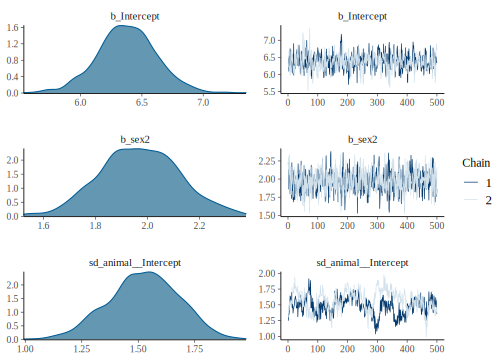
\includegraphics{wam_tuto_files/figure-latex/unnamed-chunk-60-1.pdf}
\caption{\label{fig:unnamed-chunk-60}The posterior distribution of the additive genetic effect for tarsus length in a MCMCglmm run with default values}
\end{figure}

We have constructed the prior similarly to the those in the univariate models in tutorial 1, only we are specifying a 2x2 covariance matrix rather than a single variance. In order to provide proper priors, we have set the degree of belief parameter to greater than 1 (1.002). Those priors are not necessarily weak or uninformative in all circumstances. We will consider them adequate nonetheless for this tutorial. Please the vignette of the MCMCglmm packages \citep{R-MCMCglmm} for more infomration on priors. In tutorial 1, we used full autocorrelation tables to evaluate the validity of the posterior distribution. Note that we have not done this here. For a bivariate model this table can become very complex. Nonetheless, it is worth evaluating, rather it is simply to large to include here. It can be viewed in the console as before. Here we have displayed only the autocorrelation for estimates of additive genetic effects for tarsus length with a lag of one samples (10 iterations given this MCMCglmm run with default values). This lag of 0.8457909 is clearly unacceptable. The posterior distribution of the additive genetic effect on tarsus length is shown in Figure 4 (p.~15), note the autocorrelation evident in the left-hand plot. We will opt to run the analysis for longer. This longer run could be run using the following code (including a line to save the output):

\begin{Shaded}
\begin{Highlighting}[]
\NormalTok{model2}\FloatTok{.1}\NormalTok{ <-}\StringTok{ }\KeywordTok{MCMCglmm}\NormalTok{(}\KeywordTok{cbind}\NormalTok{(bwt, tarsus) }\OperatorTok{~}\StringTok{ }\NormalTok{trait }\OperatorTok{-}\StringTok{ }\DecValTok{1}\NormalTok{,}
  \DataTypeTok{random =} \OperatorTok{~}\StringTok{ }\KeywordTok{us}\NormalTok{(trait)}\OperatorTok{:}\NormalTok{animal,}
  \DataTypeTok{rcov =} \OperatorTok{~}\StringTok{ }\KeywordTok{us}\NormalTok{(trait)}\OperatorTok{:}\NormalTok{units,}
  \DataTypeTok{family =} \KeywordTok{c}\NormalTok{(}\StringTok{"gaussian"}\NormalTok{, }\StringTok{"gaussian"}\NormalTok{),}
  \DataTypeTok{ginv =} \KeywordTok{list}\NormalTok{(}\DataTypeTok{animal =}\NormalTok{ Ainv), }\DataTypeTok{data =}\NormalTok{ gryphon,}
  \DataTypeTok{nitt =} \DecValTok{130000}\NormalTok{, }\DataTypeTok{thin =} \DecValTok{100}\NormalTok{, }\DataTypeTok{burnin =} \DecValTok{30000}\NormalTok{,}
  \DataTypeTok{prior =}\NormalTok{ prior2}\FloatTok{.1}\NormalTok{, }\DataTypeTok{verbose =} \OtherTok{FALSE}
\NormalTok{)}
\KeywordTok{save}\NormalTok{(model2}\FloatTok{.1}\NormalTok{, }\DataTypeTok{file =} \StringTok{"data/MCMCglmm_model2_1_LongRun.rda"}\NormalTok{)}
\end{Highlighting}
\end{Shaded}

However, this run might take as long as an hour. For the purpose of this tutorial we have provided an output for such a run. It can be obtained and manipulated as follows, assuming that the file \texttt{MCMCglmm\_model2\_1\_LongRun.rda} is available at the specified location:

\begin{Shaded}
\begin{Highlighting}[]
\KeywordTok{load}\NormalTok{(}\DataTypeTok{file =} \StringTok{"data/MCMCglmm_model2_1_LongRun.rda"}\NormalTok{)}
\KeywordTok{autocorr.diag}\NormalTok{(model2}\FloatTok{.1}\OperatorTok{$}\NormalTok{VCV)[, }\StringTok{"traittarsus:traittarsus.animal"}\NormalTok{][}\DecValTok{2}\NormalTok{]}
\end{Highlighting}
\end{Shaded}

\begin{verbatim}
##   Lag 100 
## 0.2608752
\end{verbatim}

This level of autocorrelation is more acceptable, at least for the purpose of demonstration in this tutorial.
We can recover variance components, heritabilities, and genetic correlations from the posterior distribution of this model:

\begin{Shaded}
\begin{Highlighting}[]
\KeywordTok{posterior.mode}\NormalTok{(model2}\FloatTok{.1}\OperatorTok{$}\NormalTok{VCV)}
\end{Highlighting}
\end{Shaded}

\begin{verbatim}
##       traitbwt:traitbwt.animal    traittarsus:traitbwt.animal 
##                       3.370616                       2.581839 
##    traitbwt:traittarsus.animal traittarsus:traittarsus.animal 
##                       2.581839                      12.463915 
##        traitbwt:traitbwt.units     traittarsus:traitbwt.units 
##                       3.761401                       2.982413 
##     traitbwt:traittarsus.units  traittarsus:traittarsus.units 
##                       2.982413                      19.556443
\end{verbatim}

\begin{Shaded}
\begin{Highlighting}[]
\NormalTok{heritability.bwt2}\FloatTok{.1}\NormalTok{ <-}\StringTok{ }\NormalTok{model2}\FloatTok{.1}\OperatorTok{$}\NormalTok{VCV[, }\StringTok{"traitbwt:traitbwt.animal"}\NormalTok{] }\OperatorTok{/}\StringTok{ }\NormalTok{(model2}\FloatTok{.1}\OperatorTok{$}\NormalTok{VCV[, }\StringTok{"traitbwt:traitbwt.animal"}\NormalTok{] }\OperatorTok{+}\StringTok{ }\NormalTok{model2}\FloatTok{.1}\OperatorTok{$}\NormalTok{VCV[, }\StringTok{"traitbwt:traitbwt.animal"}\NormalTok{])}
\KeywordTok{posterior.mode}\NormalTok{(heritability.bwt2}\FloatTok{.1}\NormalTok{)}
\end{Highlighting}
\end{Shaded}

\begin{verbatim}
##      var1 
## 0.4999336
\end{verbatim}

\begin{Shaded}
\begin{Highlighting}[]
\NormalTok{heritability.tarsus2}\FloatTok{.1}\NormalTok{ <-}\StringTok{ }\NormalTok{model2}\FloatTok{.1}\OperatorTok{$}\NormalTok{VCV[, }\StringTok{"traittarsus:traittarsus.animal"}\NormalTok{] }\OperatorTok{/}\StringTok{ }\NormalTok{(model2}\FloatTok{.1}\OperatorTok{$}\NormalTok{VCV[, }\StringTok{"traittarsus:traittarsus.animal"}\NormalTok{] }\OperatorTok{+}\StringTok{ }\NormalTok{model2}\FloatTok{.1}\OperatorTok{$}\NormalTok{VCV[, }\StringTok{"traittarsus:traittarsus.units"}\NormalTok{])}
\KeywordTok{posterior.mode}\NormalTok{(heritability.tarsus2}\FloatTok{.1}\NormalTok{)}
\end{Highlighting}
\end{Shaded}

\begin{verbatim}
##      var1 
## 0.4038754
\end{verbatim}

\begin{Shaded}
\begin{Highlighting}[]
\NormalTok{genetic.correlation2}\FloatTok{.1}\NormalTok{ <-}\StringTok{ }\NormalTok{model2}\FloatTok{.1}\OperatorTok{$}\NormalTok{VCV[, }\StringTok{"traitbwt:traittarsus.animal"}\NormalTok{] }\OperatorTok{/}\StringTok{ }\KeywordTok{sqrt}\NormalTok{(model2}\FloatTok{.1}\OperatorTok{$}\NormalTok{VCV[, }\StringTok{"traitbwt:traitbwt.animal"}\NormalTok{] }\OperatorTok{*}\StringTok{ }\NormalTok{model2}\FloatTok{.1}\OperatorTok{$}\NormalTok{VCV[, }\StringTok{"traittarsus:traittarsus.animal"}\NormalTok{])}
\KeywordTok{posterior.mode}\NormalTok{(genetic.correlation2}\FloatTok{.1}\NormalTok{)}
\end{Highlighting}
\end{Shaded}

\begin{verbatim}
##      var1 
## 0.3691503
\end{verbatim}

\hypertarget{adding-fixed-and-random-effects-1}{%
\subsection{Adding fixed and random effects}\label{adding-fixed-and-random-effects-1}}

Fixed and random effects can be added just as for the univariate case.
Given that our full model of bwt from tutorial 1 had sex as a fixed effect as well as random effects of byear and mother we could specify a bivariate formulation of this using the following code (including a line to save the output):

\begin{Shaded}
\begin{Highlighting}[]
\NormalTok{prior2}\FloatTok{.2}\NormalTok{ <-}\StringTok{ }\KeywordTok{list}\NormalTok{(}
  \DataTypeTok{G =} \KeywordTok{list}\NormalTok{(}
    \DataTypeTok{G1 =} \KeywordTok{list}\NormalTok{(}\DataTypeTok{V =} \KeywordTok{diag}\NormalTok{(}\DecValTok{2}\NormalTok{), }\DataTypeTok{nu =} \FloatTok{1.002}\NormalTok{),}
    \DataTypeTok{G2 =} \KeywordTok{list}\NormalTok{(}\DataTypeTok{V =} \KeywordTok{diag}\NormalTok{(}\DecValTok{2}\NormalTok{), }\DataTypeTok{nu =} \FloatTok{1.002}\NormalTok{),}
    \DataTypeTok{G3 =} \KeywordTok{list}\NormalTok{(}\DataTypeTok{V =} \KeywordTok{diag}\NormalTok{(}\DecValTok{2}\NormalTok{), }\DataTypeTok{nu =} \FloatTok{1.002}\NormalTok{)}
\NormalTok{  ),}
  \DataTypeTok{R =} \KeywordTok{list}\NormalTok{(}\DataTypeTok{V =} \KeywordTok{diag}\NormalTok{(}\DecValTok{2}\NormalTok{), }\DataTypeTok{nu =} \FloatTok{1.002}\NormalTok{)}
\NormalTok{)}
\NormalTok{model2}\FloatTok{.2}\NormalTok{ <-}\StringTok{ }\KeywordTok{MCMCglmm}\NormalTok{(}\KeywordTok{cbind}\NormalTok{(bwt, tarsus) }\OperatorTok{~}\StringTok{ }\NormalTok{trait }\OperatorTok{-}\StringTok{ }\DecValTok{1} \OperatorTok{+}\StringTok{ }\NormalTok{trait}\OperatorTok{:}\NormalTok{sex,}
  \DataTypeTok{random =} \OperatorTok{~}\StringTok{ }\KeywordTok{us}\NormalTok{(trait)}\OperatorTok{:}\NormalTok{animal }\OperatorTok{+}\StringTok{ }\KeywordTok{us}\NormalTok{(trait)}\OperatorTok{:}\NormalTok{byear }\OperatorTok{+}\StringTok{ }\KeywordTok{us}\NormalTok{(trait)}\OperatorTok{:}\NormalTok{mother,}
  \DataTypeTok{rcov =} \OperatorTok{~}\StringTok{ }\KeywordTok{us}\NormalTok{(trait)}\OperatorTok{:}\NormalTok{units,}
  \DataTypeTok{family =} \KeywordTok{c}\NormalTok{(}\StringTok{"gaussian"}\NormalTok{, }\StringTok{"gaussian"}\NormalTok{),}
  \DataTypeTok{ginv =} \KeywordTok{list}\NormalTok{(}\DataTypeTok{animal =}\NormalTok{ Ainv), }\DataTypeTok{data =}\NormalTok{ gryphon,}
  \DataTypeTok{nitt =} \DecValTok{130000}\NormalTok{, }\DataTypeTok{thin =} \DecValTok{100}\NormalTok{, }\DataTypeTok{burnin =} \DecValTok{30000}\NormalTok{,}
  \DataTypeTok{prior =}\NormalTok{ prior2}\FloatTok{.2}\NormalTok{, }\DataTypeTok{verbose =} \OtherTok{FALSE}
\NormalTok{)}
\KeywordTok{save}\NormalTok{(model2}\FloatTok{.2}\NormalTok{, }\DataTypeTok{file =} \StringTok{"data/MCMCglmm_model2_2_LongRun.rda"}\NormalTok{)}
\end{Highlighting}
\end{Shaded}

Again we have provided the data from one such run. It can be accessed using the code:

\begin{Shaded}
\begin{Highlighting}[]
\KeywordTok{load}\NormalTok{(}\DataTypeTok{file =} \StringTok{"data/MCMCglmm_model2_2_LongRun.rda"}\NormalTok{)}
\KeywordTok{autocorr}\NormalTok{(model2}\FloatTok{.2}\OperatorTok{$}\NormalTok{VCV)[, , }\StringTok{"traittarsus:traittarsus.animal"}\NormalTok{][}\DecValTok{3}\NormalTok{, }\DecValTok{4}\NormalTok{]}
\end{Highlighting}
\end{Shaded}

\begin{verbatim}
## [1] 0.5231926
\end{verbatim}

As before we can obtain the raw variance component estimates and genetic correlations for the random effects:

\begin{Shaded}
\begin{Highlighting}[]
\KeywordTok{posterior.mode}\NormalTok{(model2}\FloatTok{.2}\OperatorTok{$}\NormalTok{VCV)}
\end{Highlighting}
\end{Shaded}

\begin{verbatim}
##       traitbwt:traitbwt.animal    traittarsus:traitbwt.animal 
##                     1.32761860                     1.98076467 
##    traitbwt:traittarsus.animal traittarsus:traittarsus.animal 
##                     1.98076467                     0.07827994 
##        traitbwt:traitbwt.byear     traittarsus:traitbwt.byear 
##                     0.83300490                    -0.14691430 
##     traitbwt:traittarsus.byear  traittarsus:traittarsus.byear 
##                    -0.14691430                     2.79242863 
##       traitbwt:traitbwt.mother    traittarsus:traitbwt.mother 
##                     1.29299116                    -1.97967150 
##    traitbwt:traittarsus.mother traittarsus:traittarsus.mother 
##                    -1.97967150                     3.71594577 
##        traitbwt:traitbwt.units     traittarsus:traitbwt.units 
##                     2.53632072                     5.22764927 
##     traitbwt:traittarsus.units  traittarsus:traittarsus.units 
##                     5.22764927                    16.57931045
\end{verbatim}

\begin{Shaded}
\begin{Highlighting}[]
\NormalTok{genetic.correlation2}\FloatTok{.2}\NormalTok{ <-}\StringTok{ }\NormalTok{model2}\FloatTok{.2}\OperatorTok{$}\NormalTok{VCV[, }\StringTok{"traitbwt:traittarsus.animal"}\NormalTok{] }\OperatorTok{/}\StringTok{ }\KeywordTok{sqrt}\NormalTok{(model2}\FloatTok{.2}\OperatorTok{$}\NormalTok{VCV[, }\StringTok{"traitbwt:traitbwt.animal"}\NormalTok{] }\OperatorTok{*}\StringTok{ }\NormalTok{model2}\FloatTok{.2}\OperatorTok{$}\NormalTok{VCV[, }\StringTok{"traittarsus:traittarsus.animal"}\NormalTok{])}
\NormalTok{maternal.correlation2}\FloatTok{.2}\NormalTok{ <-}\StringTok{ }\NormalTok{model2}\FloatTok{.2}\OperatorTok{$}\NormalTok{VCV[, }\StringTok{"traitbwt:traittarsus.mother"}\NormalTok{] }\OperatorTok{/}\StringTok{ }\KeywordTok{sqrt}\NormalTok{(model2}\FloatTok{.2}\OperatorTok{$}\NormalTok{VCV[, }\StringTok{"traitbwt:traitbwt.mother"}\NormalTok{] }\OperatorTok{*}\StringTok{ }\NormalTok{model2}\FloatTok{.2}\OperatorTok{$}\NormalTok{VCV[, }\StringTok{"traittarsus:traittarsus.mother"}\NormalTok{])}
\KeywordTok{posterior.mode}\NormalTok{(genetic.correlation2}\FloatTok{.2}\NormalTok{)}
\end{Highlighting}
\end{Shaded}

\begin{verbatim}
##      var1 
## 0.9942065
\end{verbatim}

\begin{Shaded}
\begin{Highlighting}[]
\KeywordTok{posterior.mode}\NormalTok{(maternal.correlation2}\FloatTok{.2}\NormalTok{)}
\end{Highlighting}
\end{Shaded}

\begin{verbatim}
##       var1 
## -0.9920879
\end{verbatim}

Evaluation of the statistical support for these genetic and maternal correlations is straightforward. Because we imposed no constraint on their estimation, we can evaluate the extent to which the posterior distributions overlap zero:

\begin{Shaded}
\begin{Highlighting}[]
\KeywordTok{HPDinterval}\NormalTok{(genetic.correlation2}\FloatTok{.2}\NormalTok{, }\FloatTok{0.95}\NormalTok{)}
\end{Highlighting}
\end{Shaded}

\begin{verbatim}
##          lower     upper
## var1 0.3935369 0.9990187
## attr(,"Probability")
## [1] 0.95
\end{verbatim}

\begin{Shaded}
\begin{Highlighting}[]
\KeywordTok{HPDinterval}\NormalTok{(maternal.correlation2}\FloatTok{.2}\NormalTok{, }\FloatTok{0.95}\NormalTok{)}
\end{Highlighting}
\end{Shaded}

\begin{verbatim}
##           lower      upper
## var1 -0.9980476 -0.9443838
## attr(,"Probability")
## [1] 0.95
\end{verbatim}

Neither or these posterior distributions overlapps zero, so we can consider them both statistically supported.

\hypertarget{brms-2}{%
\section{brms}\label{brms-2}}

\begin{Shaded}
\begin{Highlighting}[]
\KeywordTok{library}\NormalTok{(brms)}
\NormalTok{Amat <-}\StringTok{ }\KeywordTok{as.matrix}\NormalTok{(nadiv}\OperatorTok{::}\KeywordTok{makeA}\NormalTok{(gryphonped))}
\NormalTok{bf_bwt <-}\StringTok{ }\KeywordTok{bf}\NormalTok{(bwt }\OperatorTok{~}\StringTok{ }\DecValTok{1} \OperatorTok{+}\StringTok{ }\NormalTok{(}\DecValTok{1} \OperatorTok{|}\StringTok{ }\NormalTok{p }\OperatorTok{|}\StringTok{ }\KeywordTok{gr}\NormalTok{(animal, }\DataTypeTok{cov =}\NormalTok{ Amat)))}
\NormalTok{bf_tarsus <-}\StringTok{ }\KeywordTok{bf}\NormalTok{(tarsus }\OperatorTok{~}\StringTok{ }\DecValTok{1} \OperatorTok{+}\StringTok{ }\NormalTok{(}\DecValTok{1} \OperatorTok{|}\StringTok{ }\NormalTok{p }\OperatorTok{|}\StringTok{ }\KeywordTok{gr}\NormalTok{(animal, }\DataTypeTok{cov =}\NormalTok{ Amat)))}
\NormalTok{brms_m2}\FloatTok{.1}\NormalTok{ <-}\StringTok{ }\KeywordTok{brm}\NormalTok{(}
\NormalTok{  bf_bwt }\OperatorTok{+}\StringTok{ }\NormalTok{bf_tarsus }\OperatorTok{+}\StringTok{ }\KeywordTok{set_rescor}\NormalTok{(}\OtherTok{TRUE}\NormalTok{),}
  \DataTypeTok{data =}\NormalTok{ gryphon,}
  \DataTypeTok{data2 =} \KeywordTok{list}\NormalTok{(}\DataTypeTok{Amat =}\NormalTok{ Amat),}
  \DataTypeTok{chains =} \DecValTok{2}\NormalTok{, }\DataTypeTok{cores =} \DecValTok{2}\NormalTok{, }\DataTypeTok{iter =} \DecValTok{1000}
\NormalTok{)}
\KeywordTok{save}\NormalTok{(brms_m2}\FloatTok{.1}\NormalTok{, }\DataTypeTok{file =} \StringTok{"data/brms_m2_1.rda"}\NormalTok{)}
\end{Highlighting}
\end{Shaded}

\begin{Shaded}
\begin{Highlighting}[]
\KeywordTok{load}\NormalTok{(}\StringTok{"data/brms_m2_1.rda"}\NormalTok{)}
\KeywordTok{summary}\NormalTok{(brms_m2}\FloatTok{.1}\NormalTok{)}
\end{Highlighting}
\end{Shaded}

\begin{verbatim}
## Warning: Parts of the model have not converged (some Rhats are > 1.05). Be
## careful when analysing the results! We recommend running more iterations and/or
## setting stronger priors.
\end{verbatim}

\begin{verbatim}
##  Family: MV(gaussian, gaussian) 
##   Links: mu = identity; sigma = identity
##          mu = identity; sigma = identity 
## Formula: bwt ~ 1 + (1 | p | gr(animal, cov = Amat)) 
##          tarsus ~ 1 + (1 | p | gr(animal, cov = Amat)) 
##    Data: gryphon (Number of observations: 683) 
## Samples: 2 chains, each with iter = 1000; warmup = 500; thin = 1;
##          total post-warmup samples = 1000
## 
## Group-Level Effects: 
## ~animal (Number of levels: 683) 
##                                     Estimate Est.Error l-95% CI u-95% CI Rhat
## sd(bwt_Intercept)                       1.81      0.21     1.41     2.20 1.06
## sd(tarsus_Intercept)                    3.44      0.43     2.49     4.25 1.05
## cor(bwt_Intercept,tarsus_Intercept)     0.38      0.14     0.08     0.62 1.02
##                                     Bulk_ESS Tail_ESS
## sd(bwt_Intercept)                         32      192
## sd(tarsus_Intercept)                      61      173
## cor(bwt_Intercept,tarsus_Intercept)      101      232
## 
## Population-Level Effects: 
##                  Estimate Est.Error l-95% CI u-95% CI Rhat Bulk_ESS Tail_ESS
## bwt_Intercept        7.49      0.16     7.20     7.79 1.00      607      839
## tarsus_Intercept    20.47      0.30    19.92    21.03 1.00      868      803
## 
## Family Specific Parameters: 
##              Estimate Est.Error l-95% CI u-95% CI Rhat Bulk_ESS Tail_ESS
## sigma_bwt        1.97      0.16     1.66     2.28 1.06       27      172
## sigma_tarsus     4.24      0.30     3.63     4.82 1.04       71      162
## 
## Residual Correlations: 
##                    Estimate Est.Error l-95% CI u-95% CI Rhat Bulk_ESS Tail_ESS
## rescor(bwt,tarsus)     0.39      0.09     0.21     0.55 1.02       95      179
## 
## Samples were drawn using sampling(NUTS). For each parameter, Bulk_ESS
## and Tail_ESS are effective sample size measures, and Rhat is the potential
## scale reduction factor on split chains (at convergence, Rhat = 1).
\end{verbatim}

\begin{Shaded}
\begin{Highlighting}[]
\KeywordTok{plot}\NormalTok{(brms_m2}\FloatTok{.1}\NormalTok{)}
\end{Highlighting}
\end{Shaded}

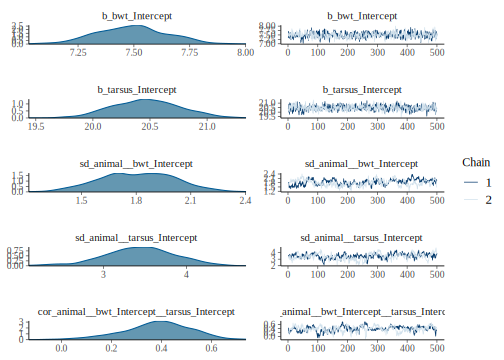
\includegraphics{wam_tuto_files/figure-latex/unnamed-chunk-69-1.pdf} 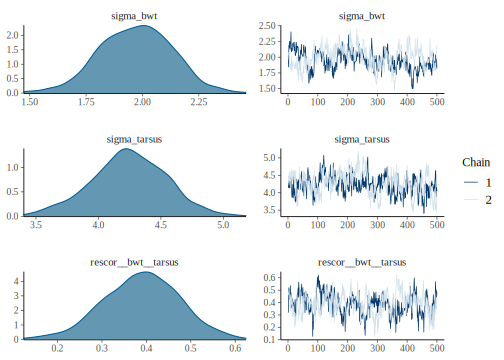
\includegraphics{wam_tuto_files/figure-latex/unnamed-chunk-69-2.pdf}

\begin{Shaded}
\begin{Highlighting}[]
\KeywordTok{VarCorr}\NormalTok{(brms_m2}\FloatTok{.1}\NormalTok{)}
\end{Highlighting}
\end{Shaded}

\begin{verbatim}
## $animal
## $animal$sd
##                  Estimate Est.Error     Q2.5    Q97.5
## bwt_Intercept    1.808171 0.2050233 1.412824 2.204805
## tarsus_Intercept 3.438368 0.4283612 2.491218 4.245264
## 
## $animal$cor
## , , bwt_Intercept
## 
##                   Estimate Est.Error       Q2.5     Q97.5
## bwt_Intercept    1.0000000 0.0000000 1.00000000 1.0000000
## tarsus_Intercept 0.3814062 0.1380014 0.07581464 0.6209038
## 
## , , tarsus_Intercept
## 
##                   Estimate Est.Error       Q2.5     Q97.5
## bwt_Intercept    0.3814062 0.1380014 0.07581464 0.6209038
## tarsus_Intercept 1.0000000 0.0000000 1.00000000 1.0000000
## 
## 
## $animal$cov
## , , bwt_Intercept
## 
##                  Estimate Est.Error      Q2.5    Q97.5
## bwt_Intercept    3.311473 0.7430185 1.9960721 4.861167
## tarsus_Intercept 2.440166 1.0901689 0.3870783 4.668720
## 
## , , tarsus_Intercept
## 
##                   Estimate Est.Error      Q2.5    Q97.5
## bwt_Intercept     2.440166  1.090169 0.3870783  4.66872
## tarsus_Intercept 12.005688  2.918741 6.2061701 18.02226
## 
## 
## 
## $residual__
## $residual__$sd
##        Estimate Est.Error     Q2.5    Q97.5
## bwt    1.970532 0.1597581 1.658782 2.276074
## tarsus 4.244704 0.2984518 3.632824 4.820109
## 
## $residual__$cor
## , , bwt
## 
##         Estimate  Est.Error      Q2.5     Q97.5
## bwt    1.0000000 0.00000000 1.0000000 1.0000000
## tarsus 0.3888754 0.08510488 0.2127907 0.5526631
## 
## , , tarsus
## 
##         Estimate  Est.Error      Q2.5     Q97.5
## bwt    0.3888754 0.08510488 0.2127907 0.5526631
## tarsus 1.0000000 0.00000000 1.0000000 1.0000000
## 
## 
## $residual__$cov
## , , bwt
## 
##        Estimate Est.Error     Q2.5    Q97.5
## bwt    3.908493 0.6282892 2.751557 5.180511
## tarsus 3.289995 0.9305960 1.572647 5.147133
## 
## , , tarsus
## 
##         Estimate Est.Error      Q2.5     Q97.5
## bwt     3.289995  0.930596  1.572647  5.147133
## tarsus 18.106495  2.530138 13.197409 23.233452
\end{verbatim}

\hypertarget{rep_measures}{%
\chapter{A repeated measures animal model}\label{rep_measures}}

This tutorial will demonstrate how to run a univariate animal model for a trait with repeated observations using different R packages and example data files provided.

\hypertarget{scenario-and-data-2}{%
\section{Scenario and data}\label{scenario-and-data-2}}

\hypertarget{scenario-2}{%
\subsection{scenario}\label{scenario-2}}

Since gryphons are iteroparous, multiple observations of reproductive traits are available for some individuals. Here we have repeated measures of lay date (measured in days after January 1) for individual females varying in age from 2 (age of maturation) up until age 6. Not all females lay every year so the number of observations per female is variable. We want to know how repeatable the trait is, and (assuming it is repeatable) how heritable it is.

\hypertarget{data-files-2}{%
\subsection{Data files}\label{data-files-2}}

The pedigree file \texttt{gryphonped.csv} is that used in the preceding tutorials but we now use a new data file \texttt{gryphonRM.csv}. Columns correspond to individual identity (\texttt{animal}), birth year (\texttt{byear}), age in years (\texttt{age}), year of measurement (\texttt{year}) and lay date (\texttt{laydate}). Each row of the data file corresponds to a single phenotypic observation. Here data are sorted by identity and then age so that the repeated observations on individuals are readily apparent. However this is not a requirement for analysis - data could equally be sorted by some other variable (\emph{e.g.}, measurement year) or be in a random order.

\begin{Shaded}
\begin{Highlighting}[]
\KeywordTok{str}\NormalTok{(gryphonRM)}
\end{Highlighting}
\end{Shaded}

\begin{verbatim}
## 'data.frame':    1607 obs. of  5 variables:
##  $ animal : Factor w/ 469 levels "1","2","3","8",..: 1 1 1 1 1 2 2 2 3 3 ...
##  $ byear  : Factor w/ 34 levels "968","970","971",..: 22 22 22 22 22 22 22 22 22 22 ...
##  $ age    : Factor w/ 5 levels "2","3","4","5",..: 1 2 3 4 5 1 2 3 1 2 ...
##  $ year   : Factor w/ 39 levels "970","971","972",..: 23 24 25 26 27 23 24 25 23 24 ...
##  $ laydate: num  19 23 24 23 29 21 17 21 20 20 ...
\end{verbatim}

\begin{Shaded}
\begin{Highlighting}[]
\KeywordTok{head}\NormalTok{(gryphonRM)}
\end{Highlighting}
\end{Shaded}

\begin{verbatim}
##   animal byear age year laydate
## 1      1   990   2  992      19
## 2      1   990   3  993      23
## 3      1   990   4  994      24
## 4      1   990   5  995      23
## 5      1   990   6  996      29
## 6      2   990   2  992      21
\end{verbatim}

\begin{verbatim}
## 'data.frame':    1309 obs. of  3 variables:
##  $ id    : int  1306 1304 1298 1293 1290 1288 1284 1283 1282 1278 ...
##  $ father: int  NA NA NA NA NA NA NA NA NA NA ...
##  $ mother: int  NA NA NA NA NA NA NA NA NA NA ...
\end{verbatim}

\begin{Shaded}
\begin{Highlighting}[]
\NormalTok{gryphonped}\OperatorTok{$}\NormalTok{id<-}\KeywordTok{as.factor}\NormalTok{(gryphonped}\OperatorTok{$}\NormalTok{id)}
\NormalTok{gryphonped}\OperatorTok{$}\NormalTok{father<-}\KeywordTok{as.factor}\NormalTok{(gryphonped}\OperatorTok{$}\NormalTok{father)}
\NormalTok{gryphonped}\OperatorTok{$}\NormalTok{mother<-}\KeywordTok{as.factor}\NormalTok{(gryphonped}\OperatorTok{$}\NormalTok{mother)}
\end{Highlighting}
\end{Shaded}

\hypertarget{asreml-r-2}{%
\section{Asreml-R}\label{asreml-r-2}}

\hypertarget{estimating-repeatability}{%
\subsection{Estimating repeatability}\label{estimating-repeatability}}

With repeated measures on individuals it is often of interest, prior to fitting a genetic model, to see how repeatable a trait is. We can estimate the repeatability of a trait as the proportion of phenotypic variance explained by individual identity.

\begin{Shaded}
\begin{Highlighting}[]
\NormalTok{modelv <-}\StringTok{ }\KeywordTok{asreml}\NormalTok{(}\DataTypeTok{fixed =}\NormalTok{ laydate }\OperatorTok{~}\StringTok{ }\DecValTok{1}\NormalTok{,}
                 \DataTypeTok{random =}\OperatorTok{~}\StringTok{ }\NormalTok{animal,}
                 \DataTypeTok{residual=}\OperatorTok{~}\KeywordTok{idv}\NormalTok{(units),}
                 \DataTypeTok{data=}\NormalTok{gryphonRM,}
                 \DataTypeTok{na.action =} \KeywordTok{na.method}\NormalTok{(}\DataTypeTok{x=}\StringTok{"omit"}\NormalTok{, }\DataTypeTok{y=}\StringTok{"omit"}\NormalTok{))}
\end{Highlighting}
\end{Shaded}

\begin{verbatim}
## Model fitted using the sigma parameterization.
## ASReml 4.1.0 Fri Feb 12 17:20:24 2021
##           LogLik        Sigma2     DF     wall    cpu
##  1     -10182.83           1.0   1606 17:20:24    0.0
##  2      -8266.10           1.0   1606 17:20:24    0.0
##  3      -6145.01           1.0   1606 17:20:24    0.0
##  4      -4651.57           1.0   1606 17:20:24    0.0
##  5      -3819.31           1.0   1606 17:20:24    0.0
##  6      -3554.22           1.0   1606 17:20:24    0.0
##  7      -3501.56           1.0   1606 17:20:24    0.0
##  8      -3497.58           1.0   1606 17:20:24    0.0
##  9      -3497.54           1.0   1606 17:20:24    0.0
## 10      -3497.54           1.0   1606 17:20:24    0.0
\end{verbatim}

Note that since we want to estimate the amount of variance explained by individual identity (rather than by additive effects), we fit \texttt{animal} as a normal random effect and we don't associate it with the pedigree.

This model partitions the phenotypic variance in \texttt{laydate} as follows:

\begin{Shaded}
\begin{Highlighting}[]
\KeywordTok{summary}\NormalTok{(modelv)}\OperatorTok{$}\NormalTok{varcomp}
\end{Highlighting}
\end{Shaded}

\begin{verbatim}
##             component std.error   z.ratio bound %ch
## animal       11.08634 1.1794319  9.399728     P   0
## units!units  21.29643 0.8896196 23.938798     P   0
## units!R       1.00000        NA        NA     F   0
\end{verbatim}

Between-individual variance is given by the \texttt{animal} component, while the residual component (\texttt{units!units}) represents within-individual variance. Here then the repeatability of the trait can be determined by hand as 0.34 (\emph{i.e.}, as 11.086/(11.086 + 21.296)).

Mean lay date might change with age, so we could ask what the repeatability of lay date is after conditioning on age. This would be done by adding \texttt{age} into the model as a fixed effect.

\begin{Shaded}
\begin{Highlighting}[]
\NormalTok{modelw <-}\StringTok{ }\KeywordTok{asreml}\NormalTok{(}\DataTypeTok{fixed =}\NormalTok{ laydate }\OperatorTok{~}\StringTok{ }\NormalTok{age,}
                 \DataTypeTok{random =}\OperatorTok{~}\StringTok{ }\NormalTok{animal,}
                 \DataTypeTok{residual=}\OperatorTok{~}\KeywordTok{idv}\NormalTok{(units),}
                 \DataTypeTok{data=}\NormalTok{gryphonRM,}
                 \DataTypeTok{na.action =} \KeywordTok{na.method}\NormalTok{(}\DataTypeTok{x=}\StringTok{"omit"}\NormalTok{, }\DataTypeTok{y=}\StringTok{"omit"}\NormalTok{))}
\end{Highlighting}
\end{Shaded}

\begin{verbatim}
## Model fitted using the sigma parameterization.
## ASReml 4.1.0 Fri Feb 12 17:20:24 2021
##           LogLik        Sigma2     DF     wall    cpu
##  1     -8402.968           1.0   1602 17:20:24    0.0
##  2     -6912.361           1.0   1602 17:20:24    0.0
##  3     -5274.379           1.0   1602 17:20:24    0.0
##  4     -4143.634           1.0   1602 17:20:24    0.0
##  5     -3541.895           1.0   1602 17:20:24    0.0
##  6     -3372.909           1.0   1602 17:20:24    0.0
##  7     -3347.670           1.0   1602 17:20:24    0.0
##  8     -3346.655           1.0   1602 17:20:24    0.0
##  9     -3346.652           1.0   1602 17:20:24    0.0
\end{verbatim}

\begin{Shaded}
\begin{Highlighting}[]
\KeywordTok{summary}\NormalTok{(modelw)}\OperatorTok{$}\NormalTok{varcomp}
\end{Highlighting}
\end{Shaded}

\begin{verbatim}
##             component std.error  z.ratio bound %ch
## animal       12.28982  1.156115 10.63027     P   0
## units!units  16.37989  0.686619 23.85586     P   0
## units!R       1.00000        NA       NA     F   0
\end{verbatim}

The repeatability of lay date, after accounting for age effects, is now estimated as 0.43 (\emph{i.e.}, as 12.29/(12.29 + 16.38)). So, just as we saw when estimating \(h^2\) in Tutorial 1, the inclusion of fixed effects will alter the estimated effect size if we determine total phenotypic variance as the sum of the variance components. Thus, proper interpretation is vital.

Here age is modelled as a 5-level factor (specified using the function \texttt{as.factor()} at the beginning of the analysis). We could equally have fitted it as a continuous variable, in which case, given potential for a late life decline, we would probably also include a quadratic term.

\hypertarget{partitioning-additive-and-permanent-environment-effects}{%
\subsection{Partitioning additive and permanent environment effects}\label{partitioning-additive-and-permanent-environment-effects}}

Generally we expect that the repeatability will set the upper limit for heritability since, while additive genetic effects will cause among-individual variation, so will other types of effects. Non-additive contributions to fixed among-individual differences are normally referred to as \emph{permanent environment effects}. If a trait has repeated measures then it is necessary to model permanent environment effects in an animal model to prevent upward bias in \(V_A\).

To illustrate this fit the animal model:

\begin{Shaded}
\begin{Highlighting}[]
\NormalTok{modelx <-}\StringTok{ }\KeywordTok{asreml}\NormalTok{(}\DataTypeTok{fixed =}\NormalTok{ laydate }\OperatorTok{~}\StringTok{ }\NormalTok{age,}
                 \DataTypeTok{random =}\OperatorTok{~}\StringTok{ }\KeywordTok{vm}\NormalTok{(animal, ainv),}
                 \DataTypeTok{residual=}\OperatorTok{~}\KeywordTok{idv}\NormalTok{(units),}
                 \DataTypeTok{data=}\NormalTok{gryphonRM,}
                 \DataTypeTok{na.action =} \KeywordTok{na.method}\NormalTok{(}\DataTypeTok{x=}\StringTok{"omit"}\NormalTok{, }\DataTypeTok{y=}\StringTok{"omit"}\NormalTok{))}
\end{Highlighting}
\end{Shaded}

\begin{verbatim}
## Model fitted using the sigma parameterization.
## ASReml 4.1.0 Fri Feb 12 17:20:24 2021
##           LogLik        Sigma2     DF     wall    cpu
##  1     -8751.390           1.0   1602 17:20:24    0.0
##  2     -7169.205           1.0   1602 17:20:24    0.0
##  3     -5427.604           1.0   1602 17:20:24    0.0
##  4     -4219.598           1.0   1602 17:20:24    0.0
##  5     -3569.815           1.0   1602 17:20:24    0.0
##  6     -3382.341           1.0   1602 17:20:24    0.0
##  7     -3352.867           1.0   1602 17:20:24    0.0
##  8     -3351.565           1.0   1602 17:20:24    0.0
##  9     -3351.560           1.0   1602 17:20:24    0.0
\end{verbatim}

Variance components are almost unchanged:

\begin{Shaded}
\begin{Highlighting}[]
\KeywordTok{summary.asreml}\NormalTok{(modelx)}\OperatorTok{$}\NormalTok{varcomp}
\end{Highlighting}
\end{Shaded}

\begin{verbatim}
##                  component std.error   z.ratio bound %ch
## vm(animal, ainv)  13.91784  1.443968  9.638607     P   0
## units!units       16.84008  0.707365 23.806768     P   0
## units!R            1.00000        NA        NA     F   0
\end{verbatim}

This suggests that all of the among-individual variance is -- rightly or wrongly -- being partitioned as \(V_A\) here. To instead obtain an unbiased estimate of \(V_A\) we need to allow for both additive genetic \emph{and} non-genetic sources of individual variation. We do this by fitting \texttt{animal} twice, once with a pedigree, and once without a pedigree (using \texttt{ide()}).

\begin{Shaded}
\begin{Highlighting}[]
\NormalTok{modely <-}\StringTok{ }\KeywordTok{asreml}\NormalTok{(}\DataTypeTok{fixed =}\NormalTok{ laydate }\OperatorTok{~}\StringTok{ }\NormalTok{age,}
                 \DataTypeTok{random =}\OperatorTok{~}\StringTok{ }\KeywordTok{vm}\NormalTok{(animal, ainv) }\OperatorTok{+}\StringTok{ }\KeywordTok{ide}\NormalTok{(animal),}
                 \DataTypeTok{residual=}\OperatorTok{~}\KeywordTok{idv}\NormalTok{(units),}
                 \DataTypeTok{data=}\NormalTok{gryphonRM,}
                 \DataTypeTok{na.action =} \KeywordTok{na.method}\NormalTok{(}\DataTypeTok{x=}\StringTok{"omit"}\NormalTok{, }\DataTypeTok{y=}\StringTok{"omit"}\NormalTok{))}
\end{Highlighting}
\end{Shaded}

\begin{verbatim}
## Model fitted using the sigma parameterization.
## ASReml 4.1.0 Fri Feb 12 17:20:24 2021
##           LogLik        Sigma2     DF     wall    cpu
##  1     -7731.394           1.0   1602 17:20:24    0.0
##  2     -6426.548           1.0   1602 17:20:24    0.0
##  3     -4997.252           1.0   1602 17:20:24    0.0
##  4     -4018.486           1.0   1602 17:20:24    0.0
##  5     -3504.988           1.0   1602 17:20:24    0.0
##  6     -3363.160           1.0   1602 17:20:24    0.0
##  7     -3341.611           1.0   1602 17:20:24    0.0
##  8     -3340.682           1.0   1602 17:20:24    0.0
##  9     -3340.679           1.0   1602 17:20:24    0.0
\end{verbatim}

\begin{Shaded}
\begin{Highlighting}[]
\KeywordTok{summary}\NormalTok{(modely)}\OperatorTok{$}\NormalTok{varcomp}
\end{Highlighting}
\end{Shaded}

\begin{verbatim}
##                  component std.error   z.ratio bound %ch
## vm(animal, ainv)  4.876101 1.8087709  2.695809     P   0
## ide(animal)       7.400983 1.7280113  4.282948     P   0
## units!units      16.380188 0.6866189 23.856300     P   0
## units!R           1.000000        NA        NA     F   0
\end{verbatim}

The estimate of \(V_A\) is now much lower since the additive and permanent environment effects are being properly separated. We can estimate \(h^2\) and the repeatability from this model:

\begin{Shaded}
\begin{Highlighting}[]
\KeywordTok{vpredict}\NormalTok{(modely, h2 }\OperatorTok{~}\StringTok{ }\NormalTok{V1}\OperatorTok{/}\NormalTok{(V1}\OperatorTok{+}\NormalTok{V2}\OperatorTok{+}\NormalTok{V3))}
\end{Highlighting}
\end{Shaded}

\begin{verbatim}
##     Estimate         SE
## h2 0.1701523 0.06073974
\end{verbatim}

\begin{Shaded}
\begin{Highlighting}[]
\KeywordTok{vpredict}\NormalTok{(modely, repeatability }\OperatorTok{~}\StringTok{ }\NormalTok{(V1}\OperatorTok{+}\NormalTok{V2)}\OperatorTok{/}\NormalTok{(V1}\OperatorTok{+}\NormalTok{V2}\OperatorTok{+}\NormalTok{V3))}
\end{Highlighting}
\end{Shaded}

\begin{verbatim}
##                Estimate         SE
## repeatability 0.4284108 0.02741602
\end{verbatim}

\hypertarget{adding-additional-effects-and-testing-significance}{%
\subsection{Adding additional effects and testing significance}\label{adding-additional-effects-and-testing-significance}}

Models of repeated measures can be extended to include other fixed or random effects. For example try including year of measurement (\texttt{year}) and birth year (\texttt{byear}) as random effects.

\begin{Shaded}
\begin{Highlighting}[]
\NormalTok{modelz <-}\StringTok{ }\KeywordTok{asreml}\NormalTok{(}\DataTypeTok{fixed =}\NormalTok{ laydate }\OperatorTok{~}\StringTok{ }\NormalTok{age,}
                 \DataTypeTok{random =}\OperatorTok{~}\StringTok{ }\KeywordTok{vm}\NormalTok{(animal, ainv) }\OperatorTok{+}\StringTok{ }\KeywordTok{ide}\NormalTok{(animal) }\OperatorTok{+}
\StringTok{                 }\NormalTok{year }\OperatorTok{+}\StringTok{ }\NormalTok{byear,}
                 \DataTypeTok{residual=}\OperatorTok{~}\KeywordTok{idv}\NormalTok{(units),}
                 \DataTypeTok{data=}\NormalTok{gryphonRM,}
                 \DataTypeTok{na.action =} \KeywordTok{na.method}\NormalTok{(}\DataTypeTok{x=}\StringTok{"omit"}\NormalTok{, }\DataTypeTok{y=}\StringTok{"omit"}\NormalTok{))}
\end{Highlighting}
\end{Shaded}

\begin{verbatim}
## Model fitted using the sigma parameterization.
## ASReml 4.1.0 Fri Feb 12 17:20:24 2021
##           LogLik        Sigma2     DF     wall    cpu
##  1     -4650.748           1.0   1602 17:20:24    0.0
##  2     -4088.264           1.0   1602 17:20:24    0.0
##  3     -3494.147           1.0   1602 17:20:24    0.0
##  4     -3127.161           1.0   1602 17:20:25    0.0 (1 restrained)
##  5     -2976.449           1.0   1602 17:20:25    0.0 (1 restrained)
##  6     -2955.785           1.0   1602 17:20:25    0.0 (1 restrained)
##  7     -2955.097           1.0   1602 17:20:25    0.0 (1 restrained)
##  8     -2955.095           1.0   1602 17:20:25    0.0 (1 restrained)
##  9     -2955.095           1.0   1602 17:20:25    0.0
\end{verbatim}

\begin{Shaded}
\begin{Highlighting}[]
\KeywordTok{summary}\NormalTok{(modelz)}\OperatorTok{$}\NormalTok{varcomp}
\end{Highlighting}
\end{Shaded}

\begin{verbatim}
##                     component std.error   z.ratio bound %ch
## byear            1.650876e-07        NA        NA     B   0
## year             7.938576e+00 1.9344619  4.103765     P   0
## vm(animal, ainv) 4.815136e+00 1.6682351  2.886365     P   0
## ide(animal)      8.433325e+00 1.5495778  5.442337     P   0
## units!units      7.795560e+00 0.3324411 23.449443     P   0
## units!R          1.000000e+00        NA        NA     F   0
\end{verbatim}

This model will return additional variance components corresponding to variation in lay dates between years of measurement and between birth cohorts of females. \(V_{byear}\) is very low and if you compare this model to a reduced model with byear excluded the log-likelihood remains unchanged.

\texttt{year} effects could alternatively be included as fixed effects (try this!). This will reduce \(V_R\) and increase the estimates of heritability and repeatability, which must now be interpreted as proportions of phenotypic variance after conditioning on both age and year of measurement effects.

\hypertarget{gremlin-3}{%
\section{gremlin}\label{gremlin-3}}

\hypertarget{mcmcglmm-3}{%
\section{MCMCglmm}\label{mcmcglmm-3}}

\hypertarget{estimating-repeatability-1}{%
\subsection{Estimating repeatability}\label{estimating-repeatability-1}}

With repeated measures on individuals it is often of interest, prior to fitting a genetic model, to see how repeatable a trait is. We can estimate the repeatability of a trait as the proportion of phenotypic variance explained by individual identity using the commands below

\begin{Shaded}
\begin{Highlighting}[]
\NormalTok{p.var <-}\StringTok{ }\KeywordTok{var}\NormalTok{(gryphonRM}\OperatorTok{$}\NormalTok{laydate, }\DataTypeTok{na.rm =} \OtherTok{TRUE}\NormalTok{)}
\NormalTok{prior3}\FloatTok{.1}\NormalTok{ <-}\StringTok{ }\KeywordTok{list}\NormalTok{(}\DataTypeTok{G =} \KeywordTok{list}\NormalTok{(}\DataTypeTok{G1 =} \KeywordTok{list}\NormalTok{(}\DataTypeTok{V =} \DecValTok{1}\NormalTok{, }\DataTypeTok{nu =} \FloatTok{0.002}\NormalTok{)), }\DataTypeTok{R =} \KeywordTok{list}\NormalTok{(}\DataTypeTok{V =} \DecValTok{1}\NormalTok{,}
\DataTypeTok{nu =} \FloatTok{0.002}\NormalTok{))}
\NormalTok{model3}\FloatTok{.1}\NormalTok{ <-}\StringTok{ }\KeywordTok{MCMCglmm}\NormalTok{(laydate }\OperatorTok{~}\StringTok{ }\DecValTok{1}\NormalTok{, }\DataTypeTok{random =} \OperatorTok{~}\StringTok{ }\NormalTok{animal, }\DataTypeTok{data =}\NormalTok{ gryphonRM,}
\DataTypeTok{prior =}\NormalTok{ prior3}\FloatTok{.1}\NormalTok{, }\DataTypeTok{verbose =} \OtherTok{FALSE}\NormalTok{)}
\KeywordTok{posterior.mode}\NormalTok{(model3}\FloatTok{.1}\OperatorTok{$}\NormalTok{VCV)}
\end{Highlighting}
\end{Shaded}

\begin{verbatim}
##   animal    units 
## 10.87766 20.78441
\end{verbatim}

Note the use of the term \texttt{animal}, since neither the \texttt{pedigree} nor the \texttt{ginv} argument are provided, it represents the between-individual variance, while the residual compo- nent (Variance) therefore represents within-individual variance. Here then the repeata- bility of the trait can be determined by as 0.353 (i.e., 11.4532/(11.4532+21.1432). Given that we set up the simulation such that mean lay date changes with age (initially increas- ing to age 5 before a late life decline) we might ask what the repeatability of lay date is after conditioning on age effect. This would be done by adding age into the model as a fixed effect.

\begin{Shaded}
\begin{Highlighting}[]
\NormalTok{model3}\FloatTok{.2}\NormalTok{ <-}\StringTok{ }\KeywordTok{MCMCglmm}\NormalTok{(laydate }\OperatorTok{~}\StringTok{ }\NormalTok{age, }\DataTypeTok{random =} \OperatorTok{~}\StringTok{ }\NormalTok{animal, }\DataTypeTok{data =}\NormalTok{ gryphonRM,}
\DataTypeTok{prior =}\NormalTok{ prior3}\FloatTok{.1}\NormalTok{, }\DataTypeTok{verbose =} \OtherTok{FALSE}\NormalTok{)}
\KeywordTok{plot}\NormalTok{(model3}\FloatTok{.2}\OperatorTok{$}\NormalTok{Sol)}
\end{Highlighting}
\end{Shaded}

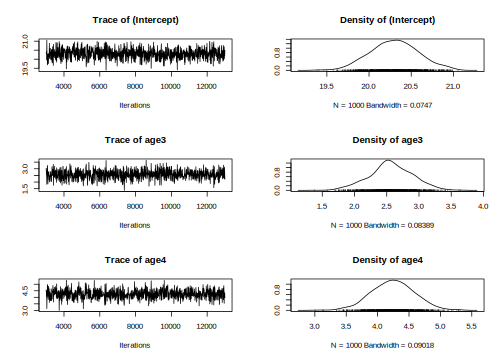
\includegraphics{wam_tuto_files/figure-latex/unnamed-chunk-83-1.pdf} 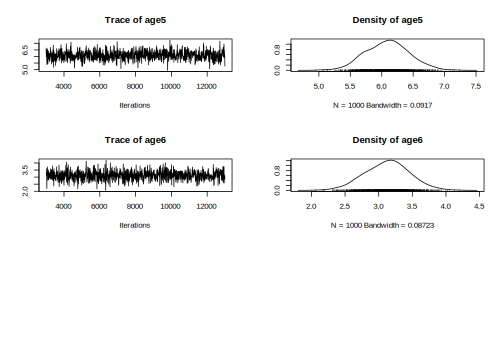
\includegraphics{wam_tuto_files/figure-latex/unnamed-chunk-83-2.pdf}

\begin{Shaded}
\begin{Highlighting}[]
\KeywordTok{plot}\NormalTok{(model3}\FloatTok{.2}\OperatorTok{$}\NormalTok{VCV)}
\end{Highlighting}
\end{Shaded}

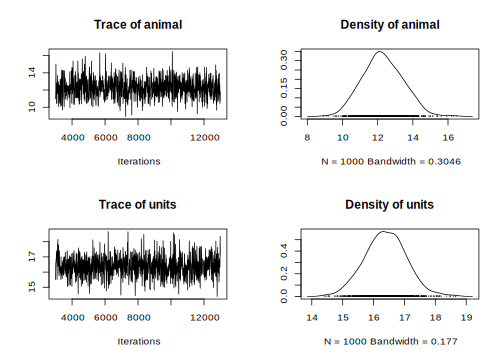
\includegraphics{wam_tuto_files/figure-latex/unnamed-chunk-83-3.pdf}

\begin{Shaded}
\begin{Highlighting}[]
\KeywordTok{posterior.mode}\NormalTok{(model3}\FloatTok{.2}\OperatorTok{$}\NormalTok{VCV)}
\end{Highlighting}
\end{Shaded}

\begin{verbatim}
##   animal    units 
## 11.95532 16.35622
\end{verbatim}

Note that the random effect structure has remained unchaged, and so we have not modified the prior between models 3.1 and 3.2. So that the repeatability of laydate, after accounting for age effects, is now estimated as 0.445 (i.e., 12.6379/(12.6379+16.465). So, just as we saw when estimating h 2 in tutorial 1, the inclusion of fixed effects will alter the estimated effect size if we determine total phenotypic variance as the sum of the variance components. Thus, proper interpretation is vital.

Here age is modelled as a 5 level factor (see the convertion of age to a factor in section 3.2). We could equally have fitted it as a continuous variable instead in which case, given the late life decline, we would probably also include a quadratic term.

\hypertarget{partitioning-additive-and-permanent-environment-effects-1}{%
\subsection{Partitioning additive and permanent environment effects}\label{partitioning-additive-and-permanent-environment-effects-1}}

Generally we expect that the repeatability will set the upper limit for heritability since, while additive genetic effects will cause among-individual variation, so will other types of effect. Non-additive contributions to fixed among-individual differences are normally referred to as `permanent environment effects', although `non-heritable effects' that are consistent within individuals may be a better way to think of modelling this effect. If a trait has repeated measures then it is necessary to model permanent environment effects in an animal model to prevent upward bias in V A . To illustrate this fit the animal model

\begin{Shaded}
\begin{Highlighting}[]
\NormalTok{Ainv <-}\StringTok{ }\KeywordTok{inverseA}\NormalTok{(gryphonped)}\OperatorTok{$}\NormalTok{Ainv}
\NormalTok{model3}\FloatTok{.3}\NormalTok{ <-}\StringTok{ }\KeywordTok{MCMCglmm}\NormalTok{(laydate }\OperatorTok{~}\StringTok{ }\DecValTok{1} \OperatorTok{+}\StringTok{ }\NormalTok{age, }\DataTypeTok{random =} \OperatorTok{~}\StringTok{ }\NormalTok{animal, }\DataTypeTok{ginv =} \KeywordTok{list}\NormalTok{(}\DataTypeTok{animal =}\NormalTok{ Ainv),}
  \DataTypeTok{data =}\NormalTok{ gryphonRM, }\DataTypeTok{prior =}\NormalTok{ prior3}\FloatTok{.1}\NormalTok{, }\DataTypeTok{verbose =} \OtherTok{FALSE}\NormalTok{)}
\KeywordTok{posterior.mode}\NormalTok{(model3}\FloatTok{.3}\OperatorTok{$}\NormalTok{VCV)}
\end{Highlighting}
\end{Shaded}

\begin{verbatim}
##   animal    units 
## 13.48495 17.16223
\end{verbatim}

This suggests that all of the among-individual variance is - rightly or wrongly - being partitioned as V A here. In fact here the partition is wrong since the simulation included both additive genetic effects and additional fixed heterogeneity that was not associated with the pedigree structure (i.e.~permanent environment effects).
In order to fit both permanent environemnt and additive genetic effects, we need to fit the individual identity twice in the model: once linked to the pedigree (genetic effect) and once not linked to the pedigree (permanenet environemnt effect).
To do so, we need to duplicate the variable containing the individual identity and give it a new name.
An more appropriate estimate of V A is given by the model:

\begin{Shaded}
\begin{Highlighting}[]
\NormalTok{gryphonRM}\OperatorTok{$}\NormalTok{animal_pe <-}\StringTok{ }\NormalTok{gryphonRM}\OperatorTok{$}\NormalTok{animal}
\NormalTok{p.var <-}\StringTok{ }\KeywordTok{var}\NormalTok{(gryphonRM}\OperatorTok{$}\NormalTok{laydate, }\DataTypeTok{na.rm =} \OtherTok{TRUE}\NormalTok{)}
\NormalTok{prior3}\FloatTok{.4}\NormalTok{ <-}\StringTok{ }\KeywordTok{list}\NormalTok{(}\DataTypeTok{G =} \KeywordTok{list}\NormalTok{(}\DataTypeTok{G1 =} \KeywordTok{list}\NormalTok{(}\DataTypeTok{V =} \DecValTok{1}\NormalTok{, }\DataTypeTok{nu =} \FloatTok{0.002}\NormalTok{), }\DataTypeTok{G2 =} \KeywordTok{list}\NormalTok{(}\DataTypeTok{V =} \DecValTok{1}\NormalTok{,}
\DataTypeTok{nu =} \FloatTok{0.002}\NormalTok{)), }\DataTypeTok{R =} \KeywordTok{list}\NormalTok{(}\DataTypeTok{V =} \DecValTok{1}\NormalTok{, }\DataTypeTok{nu =} \FloatTok{0.002}\NormalTok{))}
\NormalTok{model3}\FloatTok{.4}\NormalTok{ <-}\StringTok{ }\KeywordTok{MCMCglmm}\NormalTok{(laydate }\OperatorTok{~}\StringTok{ }\DecValTok{1} \OperatorTok{+}\StringTok{ }\NormalTok{age, }\DataTypeTok{random =} \OperatorTok{~}\NormalTok{animal }\OperatorTok{+}\StringTok{ }\NormalTok{animal_pe,}
\DataTypeTok{ginv =} \KeywordTok{list}\NormalTok{(}\DataTypeTok{animal =}\NormalTok{ Ainv), }\DataTypeTok{data =}\NormalTok{ gryphonRM, }\DataTypeTok{prior =}\NormalTok{ prior3}\FloatTok{.4}\NormalTok{, }\DataTypeTok{verbose =} \OtherTok{FALSE}\NormalTok{)}
\KeywordTok{posterior.mode}\NormalTok{(model3}\FloatTok{.4}\OperatorTok{$}\NormalTok{VCV)}
\end{Highlighting}
\end{Shaded}

\begin{verbatim}
##    animal animal_pe     units 
##  4.792356  7.586770 16.585880
\end{verbatim}

The estimate of V A is now much lower (reduced from 13.6735 to 5.1238) since the ad- ditive and permanent environment effects are being properly separated. We could obtain estimates of h 2 and of the repeatability from this model using the following commands:

\begin{Shaded}
\begin{Highlighting}[]
\NormalTok{model3.}\FloatTok{4.}\NormalTok{VP <-}\StringTok{ }\NormalTok{model3}\FloatTok{.4}\OperatorTok{$}\NormalTok{VCV[, }\StringTok{"animal"}\NormalTok{] }\OperatorTok{+}\StringTok{ }\NormalTok{model3}\FloatTok{.4}\OperatorTok{$}\NormalTok{VCV[, }\StringTok{"animal_pe"}\NormalTok{] }\OperatorTok{+}\StringTok{ }\NormalTok{model3}\FloatTok{.4}\OperatorTok{$}\NormalTok{VCV[, }\StringTok{"units"}\NormalTok{]}
\NormalTok{model3.}\FloatTok{4.}\NormalTok{PE_VA <-}\StringTok{ }\NormalTok{model3}\FloatTok{.4}\OperatorTok{$}\NormalTok{VCV[, }\StringTok{"animal"}\NormalTok{] }\OperatorTok{+}\StringTok{ }\NormalTok{model3}\FloatTok{.4}\OperatorTok{$}\NormalTok{VCV[,}\StringTok{"animal_pe"}\NormalTok{]}
\KeywordTok{posterior.mode}\NormalTok{(model3.}\FloatTok{4.}\NormalTok{PE_VA}\OperatorTok{/}\NormalTok{model3.}\FloatTok{4.}\NormalTok{VP)}
\end{Highlighting}
\end{Shaded}

\begin{verbatim}
##      var1 
## 0.4163568
\end{verbatim}

\begin{Shaded}
\begin{Highlighting}[]
\KeywordTok{posterior.mode}\NormalTok{(model3}\FloatTok{.4}\OperatorTok{$}\NormalTok{VCV[, }\StringTok{"animal"}\NormalTok{]}\OperatorTok{/}\NormalTok{model3.}\FloatTok{4.}\NormalTok{VP)}
\end{Highlighting}
\end{Shaded}

\begin{verbatim}
##     var1 
## 0.159411
\end{verbatim}

\hypertarget{adding-additional-effects-and-testing-significance-1}{%
\subsection{Adding additional effects and testing significance}\label{adding-additional-effects-and-testing-significance-1}}

Models of repeated measures can be extended to include other fixed or random effects.
For example try including year of measurement (year).

\begin{Shaded}
\begin{Highlighting}[]
\NormalTok{p.var <-}\StringTok{ }\KeywordTok{var}\NormalTok{(gryphonRM}\OperatorTok{$}\NormalTok{laydate, }\DataTypeTok{na.rm =} \OtherTok{TRUE}\NormalTok{)}
\NormalTok{prior3}\FloatTok{.5}\NormalTok{ <-}\StringTok{ }\KeywordTok{list}\NormalTok{(}\DataTypeTok{G =} \KeywordTok{list}\NormalTok{(}\DataTypeTok{G1 =} \KeywordTok{list}\NormalTok{(}\DataTypeTok{V =} \DecValTok{1}\NormalTok{, }\DataTypeTok{nu =} \FloatTok{0.002}\NormalTok{), }\DataTypeTok{G2 =} \KeywordTok{list}\NormalTok{(}\DataTypeTok{V =} \DecValTok{1}\NormalTok{,}
\DataTypeTok{nu =} \FloatTok{0.002}\NormalTok{), }\DataTypeTok{G3 =} \KeywordTok{list}\NormalTok{(}\DataTypeTok{V =} \DecValTok{1}\NormalTok{, }\DataTypeTok{nu =} \FloatTok{0.002}\NormalTok{), }\DataTypeTok{G4 =} \KeywordTok{list}\NormalTok{(}\DataTypeTok{V =} \DecValTok{1}\NormalTok{,}
\DataTypeTok{nu =} \FloatTok{0.002}\NormalTok{)), }\DataTypeTok{R =} \KeywordTok{list}\NormalTok{(}\DataTypeTok{V =} \DecValTok{1}\NormalTok{, }\DataTypeTok{nu =} \FloatTok{0.002}\NormalTok{))}
\NormalTok{model3}\FloatTok{.5}\NormalTok{ <-}\StringTok{ }\KeywordTok{MCMCglmm}\NormalTok{(laydate }\OperatorTok{~}\StringTok{ }\DecValTok{1} \OperatorTok{+}\StringTok{ }\NormalTok{age, }\DataTypeTok{random =} \OperatorTok{~}\NormalTok{animal }\OperatorTok{+}\StringTok{ }\NormalTok{animal_pe }\OperatorTok{+}
\NormalTok{year }\OperatorTok{+}\StringTok{ }\NormalTok{byear, }\DataTypeTok{ginv =} \KeywordTok{list}\NormalTok{(}\DataTypeTok{animal =}\NormalTok{ Ainv), }\DataTypeTok{data =}\NormalTok{ gryphonRM, }\DataTypeTok{prior =}\NormalTok{ prior3}\FloatTok{.5}\NormalTok{,}
\DataTypeTok{verbose =} \OtherTok{FALSE}\NormalTok{)}
\KeywordTok{posterior.mode}\NormalTok{(model3}\FloatTok{.5}\OperatorTok{$}\NormalTok{VCV)}
\end{Highlighting}
\end{Shaded}

\begin{verbatim}
##     animal  animal_pe       year      byear      units 
## 5.21481674 7.87072250 7.91353832 0.00114482 7.78745344
\end{verbatim}

This model will return additional variance components corresponding to year of mea- surement effects and birth year (of the female effects). The latter were not simulated as should be apparent from the parameter estimate (and by the support interval derivable from the posterior distribution and from DIC-based comparison of model3.5 and a model from which the birth year term had been eliminated, see tutorial 1). However, year ef- fects were simulated as should be apparent from the from the modal estimate and from the support interval (try this yourself using HPDinterval()) and this could be formally confirmed by comparison of DIC. year effects could alternatively be included as fixed effects (try this, you should be able to handle the new prior specification at this point). Since we simulated large year of measurement effects this treatment will reduce V R and increase the the estimates of heritability and repeatability which must now be interpreted as proportions of phenotypic variance after conditioning on both age and year of measurement effects.

\hypertarget{brms-3}{%
\section{brms}\label{brms-3}}

\begin{Shaded}
\begin{Highlighting}[]
\KeywordTok{library}\NormalTok{(brms)}
\NormalTok{Amat <-}\StringTok{ }\NormalTok{nadiv}\OperatorTok{::}\KeywordTok{makeA}\NormalTok{(Ped)}

\NormalTok{model_simple1}\FloatTok{.1}\NormalTok{ <-}\StringTok{ }\KeywordTok{brm}\NormalTok{(}
\NormalTok{  bwt }\OperatorTok{~}\StringTok{ }\DecValTok{1} \OperatorTok{+}\StringTok{ }\NormalTok{(}\DecValTok{1}\OperatorTok{|}\NormalTok{animal) }\OperatorTok{+}\StringTok{ }\NormalTok{(}\DecValTok{1}\OperatorTok{|}\NormalTok{animal_pe), }\DataTypeTok{data =}\NormalTok{ gryphonRM,}
  \DataTypeTok{family =} \KeywordTok{gaussian}\NormalTok{(), }\DataTypeTok{cov_ranef =} \KeywordTok{list}\NormalTok{(}\DataTypeTok{animal =}\NormalTok{ Amat),}
  \DataTypeTok{chains =} \DecValTok{2}\NormalTok{, }\DataTypeTok{cores =} \DecValTok{2}\NormalTok{, }\DataTypeTok{iter =} \DecValTok{1000}
\NormalTok{)}

\KeywordTok{summary}\NormalTok{(model_simple1}\FloatTok{.1}\NormalTok{)}
\KeywordTok{plot}\NormalTok{(model_simple1}\FloatTok{.1}\NormalTok{)}
\end{Highlighting}
\end{Shaded}

\hypertarget{quick-comparison-of-codes}{%
\chapter{Quick comparison of codes}\label{quick-comparison-of-codes}}

\hypertarget{univariate-model-with-repeated-measures}{%
\section{Univariate model with repeated measures}\label{univariate-model-with-repeated-measures}}

\hypertarget{asreml-r-3}{%
\subsection{Asreml-R}\label{asreml-r-3}}

\hypertarget{gremlin-4}{%
\subsection{gremlin}\label{gremlin-4}}

\hypertarget{mcmcglmm-4}{%
\subsection{MCMCglmm}\label{mcmcglmm-4}}

\hypertarget{brms-4}{%
\subsection{brms}\label{brms-4}}

\hypertarget{bivariate-model}{%
\section{bivariate model}\label{bivariate-model}}

\hypertarget{asreml-r-4}{%
\subsection{Asreml-R}\label{asreml-r-4}}

\hypertarget{gremlin-5}{%
\subsection{gremlin}\label{gremlin-5}}

\hypertarget{mcmcglmm-5}{%
\subsection{MCMCglmm}\label{mcmcglmm-5}}

\hypertarget{brms-5}{%
\subsection{brms}\label{brms-5}}

\bibliography{book.bib,packages.bib}

\printindex

\end{document}
